\documentclass[11pt]{article}
\usepackage{amsmath, amsthm, amssymb, pdfpages} 
\usepackage{fullpage}
\usepackage{hyperref}
\usepackage{graphicx}
\usepackage[capitalize]{cleveref}
\usepackage[CaptionBefore]{fltpage} % for large figures, captions go on prev page

% options for pretty tables from CSV files
\usepackage{booktabs,csvsimple,siunitx}
% for commas in big numbers (i.e. "3,000,000")
\sisetup{group-separator={,}}

% next three for UTF8 to work (for non-ASCII names to work without awkward codes)
\usepackage[T1]{fontenc}
\usepackage{textcomp}
\usepackage[utf8]{inputenc}

% import biblatex with prefered settings
% loads biblatex with all the nice standard options that John determined some time ago!
% this version uses a ``Harvard'' style (first author last name, year in parentheses).
% also loads xpatch

% biblatex
% harvard style
\usepackage[style=authoryear,natbib,maxcitenames=2,doi=false,isbn=false,url=false,backend=bibtex]{biblatex}
% numeric style
%% \usepackage[style=numeric-comp,sorting=none,giveninits=true,
%%                      doi=false,isbn=false,url=false,backend=bibtex]{biblatex}
% remove "In: " before journal title
\renewbibmacro{in:}{}
% remove language
\AtEveryBibitem{\clearlist{language}}
% remove month
\AtEveryBibitem{\clearfield{month}}
% and also notes
\AtEveryBibitem{\clearfield{note}}
% remove dots between volume and issue
\usepackage{xpatch}
\xpatchbibmacro{volume+number+eid}{%
  \setunit*{\adddot}%
}{%
}{}{}
% put issue in parentheses
\DeclareFieldFormat[article]{number}{\mkbibparens{#1}}


\bibliography{zotero, dummy}

% path of images
\graphicspath{ {../data/} }

% define shortcuts for awkward math symbols
% this also helps us change them more easily later, if needed
\newcommand{\rmsd}{\text{SRMSD}_p}
\newcommand{\auc}{\text{AUC}_\text{PR}}

\usepackage{kinshipsymbols}

% double line spacing (PLoS wants this)
\usepackage{setspace}
\doublespacing
% original, smaller spacing
%\renewcommand{\baselinestretch}{1.2}

% cool automatic supplemental figures/tables!
% http://bytesizebio.net/2013/03/11/adding-supplementary-tables-and-figures-in-latex/
% with some additions
\newcommand{\beginsupplement}{%
  \setcounter{table}{0}
  \renewcommand{\thetable}{S\arabic{table}}%
  \setcounter{figure}{0}
  \renewcommand{\thefigure}{S\arabic{figure}}%
  \setcounter{section}{0}
  \renewcommand{\thesection}{S\arabic{section}}%
  \setcounter{equation}{0}
  \renewcommand{\theequation}{S\arabic{equation}}%
  \setcounter{page}{1}
  \renewcommand{\thepage}{S\arabic{page}}%
}


% OLD: Testing the effectiveness of principal components in adjusting for relatedness in genetic association studies
\title{\Large \textbf{
    Limitations of principal components in quantitative genetic association models for human studies
  }}
\author{Yiqi Yao$^{1,2}$, Alejandro Ochoa$^{1,3,*}$}
\date{}

\begin{document}
\maketitle

\noindent
$^1$ Department of Biostatistics and Bioinformatics, Duke University, Durham, NC 27705, USA \\
$^2$ BenHealth Consulting, Huangpu Mengzi Road 395 1-601, Shanghai, China \\
$^3$ Duke Center for Statistical Genetics and Genomics, Duke University, Durham, NC 27705, USA \\
$^*$ Corresponding author: \texttt{alejandro.ochoa@duke.edu}

\begin{abstract}
  Principal Component Analysis (PCA) and the Linear Mixed-Effects Model (LMM), sometimes in combination, are the most common modern models for genetic association.
  Previous PCA-LMM comparisons give mixed results and unclear guidance, and have several limitations, including not varying the number of principal components (PCs), simulating overly simple population structures, and inconsistent use of real data and power evaluations.
  In this work, we thoroughly evaluate PCA and LMM both with varying number of PCs in new realistic genotype and complex trait simulations including admixed families, trees, and large real multiethnic human genotype datasets (1000 Genomes Project, the Human Genome Diversity Panel, and Human Origins) with simulated traits.
  We find that LMM without PCs performs best in all cases, with the largest effects in the family simulation and all real human datasets.
  We determined that the large gaps in PCA to LMM performance on the real human datasets is due to the high-dimensional family structure stemming from large numbers of distant relatives, and not from the smaller number of highly related pairs.
  While it was known that PCA fails on family data, here we report a strong effect on association of cryptic family relatedness in several genetically diverse human datasets, a problem that is not avoided with the common practice of pruning high-relatedness individual pairs.
  Overall, this work better characterizes the severe limitations of PCA compared to LMM in modeling the complex relatedness structures present in real multiethnic human data and its impact in association studies.
\end{abstract}

% used for ASHG abstract
% \textbf{Keywords:} genetic association, statistical genetics, population structure, complex traits, genetic diversity.

\textbf{Abbreviations:}
PCA: principal component analysis;
PCs: principal components;
LMM: linear mixed-effects model;
FES: fixed effect sizes;
RC: random coefficients;
MAF: minor allele frequency;
WGS: whole genome sequencing.

\section{Introduction} 

% need for specialized approaches
The goal of a genetic association study is to identify loci whose genotype variation is significantly correlated to given trait.
Naive association tests assume that genotypes are drawn independently from a common allele frequency.
This assumption does not hold for structured populations, which includes multiethnic cohorts and admixed individuals (ancient relatedness), and for family data (recent relatedness) \citep{astle_population_2009}.
When insufficient approaches are applied to data with relatedness, their association statistics are miscalibrated, resulting in excess false positives and loss of power \citep{devlin_genomic_1999, voight_confounding_2005, astle_population_2009}.
Therefore, many specialized approaches have been developed for genetic association under relatedness, of which PCA and LMM are the most popular.

% PCA
Genetic association with PCA consists of including the top eigenvectors of the population kinship matrix as covariates in a generalized linear model \citep{zhang_semiparametric_2003, price_principal_2006, bouaziz_accounting_2011}.
These top eigenvectors are commonly referred to as PCs in genetics \citep{patterson_population_2006}, the convention adopted here, but in other fields PCs denote the projections of loci onto eigenvectors \citep{jolliffe_principal_2002}.
The direct ancestor of PCA association is structured association, in which inferred ancestry or admixture proportions are used as regression covariates \citep{pritchard_association_2000}.
These models are deeply connected because PCs map to ancestry empirically \citep{alexander_fast_2009, zhou_strong_2016} and theoretically \citep{mcvean_genealogical_2009,zheng_eigenanalysis_2016,cabreros_likelihood-free_2019,chiu_inferring_2022}, and they work as well as global ancestry in association studies but are estimated more easily \citep{patterson_population_2006, zhao_arabidopsis_2007, alexander_fast_2009, bouaziz_accounting_2011}.
The strength of PCA is its simplicity, which as covariates can be readily included in more complex models, such as haplotype association \citep{xu_detecting_2014} and polygenic models \citep{qian_fast_2020}.
However, PCA assumes that relatedness is low-dimensional, which may limit its applicability.
PCA is known to be inadequate for family data \citep{patterson_population_2006, thornton_roadtrips:_2010, price_new_2010}, which is called ``cryptic relatedness'' when it is unknown to the researchers, but no other troublesome cases have been confidently identified.
Recent work has focused on developing more scalable versions of the PCA algorithm \citep{lee_sparse_2012, abraham_fast_2014, galinsky_fast_2016, abraham_flashpca2:_2017, agrawal_scalable_2020}.
PCA remains a popular and powerful approach for association studies.

% LMM
The other dominant association model under relatedness is the LMM, which includes a random effect parametrized by the kinship matrix.
Unlike PCA, LMM does not assume that relatedness is low-dimensional, and explicitly models families via the kinship matrix.
Early LMMs required kinship matrices estimated from known pedigrees or which otherwise captured recent relatedness only \citep{yu_unified_2006, zhao_arabidopsis_2007}.
Modern LMMs estimate kinship from genotypes using a non-parametric estimator, often referred to as a genetic relationship matrix, that captures the combined covariance due to recent family relatedness and ancestral population structure \citep{kang_efficient_2008, astle_population_2009, ochoa_estimating_2021}.
The classic LMM assumes a quantitative (continuous) complex trait, the focus of our work.
Although case-control (binary) traits and their underlying ascertainment are theoretically a challenge \citep{yang_advantages_2014}, LMMs have been applied successfully to balanced case-control studies \citep{astle_population_2009, kang_variance_2010} and simulations \citep{price_new_2010, wu_comparison_2011, sul_mixed_2013}, and have been adapted for unbalanced case-control studies \citep{zhou_efficiently_2018}.
However, LMMs tend to be considerably slower than PCA and other models, so much effort has focused on improving their runtime and scalability \citep{aulchenko_genomewide_2007, kang_efficient_2008, kang_variance_2010, zhang_mixed_2010, lippert_fast_2011, yang_gcta:_2011, listgarten_improved_2012, zhou_genome-wide_2012, svishcheva_rapid_2012, loh_efficient_2015, zhou_efficiently_2018}.

% LMM+PCA
An LMM variant that incorporates PCs as fixed covariates is tested thoroughly in our work.
Since PCs are the top eigenvectors of the same kinship matrix estimate used in modern LMMs \citep{astle_population_2009, hoffman_correcting_2013}, then population structure is modeled twice in an LMM with PCs.
However, some previous work has found the apparent redundancy of an LMM with PCs beneficial \citep{price_new_2010, tucker_improving_2014}, while others did not \citep{liu_controlling_2011}, and the approach continues to be used \citep{zeng_signatures_2018}.
Recall that early LMMs used kinship to model family relatedness only, so population structure had to be modeled separately, in practice as admixture fractions instead of PCs \citep{yu_unified_2006, zhao_arabidopsis_2007}.

\begin{table}[b!]
  \centering
  \small
  \caption{
    \textbf{Previous PCA-LMM evaluations in the literature.}
  }
  \label{tab:lit}
  \begin{tabular}{l|ccc|ccccc}
    \toprule
                & \multicolumn{3}{c|}{Sim. Genotypes} & \\
    Publication & Type\textsuperscript{a} & $K$\textsuperscript{b} & \Fst\textsuperscript{c} & Real\textsuperscript{d} & Trait\textsuperscript{e} & Power & PCs ($r$) & Best \\
    \midrule
    % Publication                    & Sim &    K &     Fst &       Re & Ph &      Pow & PCAr & Best\\
    \textcite{zhao_arabidopsis_2007} &     &      &         &\checkmark&  Q &\checkmark&    8 & LMM \\
    \textcite{astle_population_2009} &   I &    3 &    0.10 &          & CC &\checkmark&   10 & Tie \\
    \textcite{kang_variance_2010}    &     &      &         &\checkmark&Both&          &2-100 & LMM \\
    \textcite{price_new_2010}        &I, F &    2 &    0.01 &          & CC &          &    1 & Mixed \\
    \textcite{wu_comparison_2011}    &I, A &  2-4 &    0.01 &          & CC &\checkmark&   10 & Mixed \\
    \textcite{liu_controlling_2011}  &S, A &  2-3 &       R &          &  Q &\checkmark&   10 & Tie \\
    \textcite{sul_mixed_2013}        &   I &    2 &    0.01 &          & CC &          &    1 & Tie \\
    \textcite{tucker_improving_2014} &   I &    2 &    0.05 &\checkmark&Both&\checkmark&    5 & Tie \\
    \textcite{yang_advantages_2014}  &     &      &         &\checkmark& CC &\checkmark&    5 & Tie \\
    \textcite{song_testing_2015}     &S, A &  2-3 &       R &          &  Q &          &    3 & LMM \\
    \textcite{loh_efficient_2015}    &     &      &         &\checkmark&  Q &\checkmark&   10 & LMM \\
    \textcite{liu_iterative_2016}    &     &      &         &\checkmark&  Q &\checkmark&  3-6 & LMM \\ 
    \textcite{sul_population_2018}   &     &      &         &\checkmark&  Q &          &  100 & LMM \\
    This work                        &A, T, F&10-243&$\le$0.25&\checkmark&  Q &\checkmark& 0-90 & LMM \\
    \bottomrule
  \end{tabular}
  \begin{flushleft} 
    \textsuperscript{a}Genotype simulation types. I: Independent subpopulations; S: subpopulations (with parameters drawn from real data); A: Admixture; T: Tree; F: Family.\\
    \textsuperscript{b}Model dimensionality (number of subpopulations or ancestries)\\
    \textsuperscript{c}R: simulated parameters based on real data, \Fst not reported.\\
    \textsuperscript{d}Evaluations using unmodified real genotypes.\\
    \textsuperscript{e}Q: quantitative; CC: case-control.
  \end{flushleft}
\end{table}


% LMM and PCA are similar
LMM and PCA are closely related models \citep{astle_population_2009, hoffman_correcting_2013}, so similar performance is expected particularly under low-dimensional relatedness.
Direct comparisons have yielded mixed results, with several studies finding superior performance for LMM (notably from papers promoting advances in LMMs) while many others report comparable performance (\cref{tab:lit}).
No papers find that PCA outperforms LMM decisively, although PCA occasionally performs better in isolated and artificial cases or individual measures (often with unknown significance).
Previous studies were generally divided those that employed simulated versus real genotypes (only one study used both).
The simulated genotype studies, which tended to have low dimensionalities and differentiation (\Fst), were more likely to report ties or mixed results (6/7), whereas real genotypes tended to clearly favor LMMs (5/7).
Similarly, 6/8 papers with quantitative traits favor LMMs, whereas 5/7 papers with case-control traits gave ties or mixed results (the only factor we do not explore).
Additionally, although all previous evaluations measured type I error (or proxies such as inflation factors or QQ plots), a large fraction (5/13) did not measure power (including proxies such as ROC curves), and only two used more than one number of PCs for PCA.
Lastly, no consensus has emerged as to why LMM might outperform PCA or vice versa \citep{price_new_2010, sul_mixed_2013, price_response_2013, hoffman_correcting_2013}, or which features of the real datasets are critical for the LMM advantage other than cryptic relatedness, resulting in unclear guidance for using PCA.
Hence, our work includes real and simulated genotypes with higher dimensionalities and differentiation matching that of multiethnic human cohorts, we vary the number of PCs, and measure robust proxies for type I error control and power.

% this work
In this work, we evaluate the PCA and LMM association models under various numbers of PCs (included in LMM too).
We use genotype simulations (admixture, family, and tree models) and three real datasets: the 1000 Genomes Project \citep{the_1000_genomes_project_consortium_map_2010, 1000_genomes_project_consortium_integrated_2012}, the Human Genome Diversity Panel (HGDP) \citep{cann_human_2002, rosenberg_genetic_2002, bergstrom_insights_2020}, and Human Origins \citep{patterson_ancient_2012, lazaridis_ancient_2014, lazaridis_genomic_2016, skoglund_genomic_2016}.
We simulate quantitative traits from two models: fixed effect sizes (FES; coefficients inverse to allele frequency) that matches real data \citep{park_distribution_2011, zeng_signatures_2018, oconnor_extreme_2019} and corresponds to high pleiotropy and strong balancing selection \citep{simons_population_2018} and strong negative selection \citep{zeng_signatures_2018, oconnor_extreme_2019}, which are appropriate assumptions for diseases; and random coefficients (RC; independent of allele frequency) that corresponds to neutral traits \citep{zeng_signatures_2018, simons_population_2018}.
LMM without PCs consistently performs best, and greatly outperforms PCA in the family simulation and in all real datasets.
The tree simulations do not recapitulate the real data results, suggesting that family relatedness in real data is the reason for poor PCA performance.
Lastly, removing up to 4th degree relatives in the real datasets recapitulates poor PCA performance, showing that the more numerous distant relatives explain the result, and suggesting that PCA is generally not an appropriate model for real data.
All together, we find that LMMs without PCs are generally a preferable association model, and present novel simulation and evaluation approaches to measure the performance of these and other genetic association approaches.

\section{Materials and Methods}

\subsection{The complex trait model and PCA and LMM approximations}

Let $\xij \in \{ 0, 1, 2 \}$ be the genotype at the biallelic locus $i$ for individual $j$, which counts the number of reference alleles.
Suppose there are $n$ individuals and $m$ loci,
$\mathbf{X} = ( \xij )$ is their $m \times n$ genotype matrix, and
$\mathbf{y}$ is the length-$n$ (column) vector of individual trait values.
The additive linear model for a quantitative (continuous) trait is:
\begin{equation}
  \label{eq:trait}
  \mathbf{y}
  =
  \mathbf{1} \alpha + \mathbf{X}^\intercal \boldsymbol{\beta} + \boldsymbol{\epsilon}
  ,
\end{equation}
where
$\mathbf{1}$ is a length-$n$ vector of ones,
$\alpha$ is the scalar intercept coefficient,
$\boldsymbol{\beta}$ is the length-$m$ vector of locus coefficients,
$\boldsymbol{\epsilon}$ is a length-$n$ vector of residuals,
and $\intercal$ denotes matrix transposition.
The residuals follow $\epsilon_j \sim \text{Normal}(0, \sigma^2)$ independently per individual $j$, for some $\sigma^2$.
For simplicity, non-genetic covariates are omitted from this model (and the PCA and LMM counterparts) but are trivial to include without changing any of our theoretical results.

The full model of \cref{eq:trait}, which has a coefficient for each of the $m$ loci, is overdetermined in current datasets where $m \gg n$.
The PCA and LMM models, respectively, approximate the full model fit at a single locus $i$:
\begin{align}
  \label{eq:pca_gwas}
  \text{PCA:}\quad
  \mathbf{y}
  &=
  \mathbf{1} \alpha + \mathbf{x}_i \beta_i + \mathbf{U}_r \boldsymbol{\gamma}_r + \boldsymbol{\epsilon}
  , \\
  \label{eq:lmm_gwas}
  \text{LMM:}\quad
  \mathbf{y}
  &=
  \mathbf{1} \alpha + \mathbf{x}_i \beta_i + \mathbf{s} + \boldsymbol{\epsilon}
    ,
    \quad\quad
    \mathbf{s} \sim \text{Normal} \left( \mathbf{0}, 2 \sigma^2_s \mathbf{\Phi}^T \right),
\end{align}
where $\mathbf{x}_i$ is the length-$n$ vector of genotypes at locus $i$ only,
$\beta_i$ is the locus coefficient,
$\mathbf{U}_r$ is an $n \times r$ matrix of PCs,
$\boldsymbol{\gamma}_r$ is the length-$r$ vector of PC coefficients,
$\mathbf{s}$ is a length-$n$ vector of random effects,
$\mathbf{\Phi}^T = (\kt)$ is the $n \times n$ kinship matrix conditioned on the ancestral population $T$,
and $\sigma^2_s$ is a variance factor (do not confuse the ancestral population superscript $T$ with the matrix transposition symbol $\intercal$).
Both models condition the regression of the focal locus $i$ on an approximation of the total polygenic effect $\mathbf{X}^\intercal \boldsymbol{\beta}$ with the same covariance structure, which is parametrized by the kinship matrix.
Under the kinship model, genotypes are random variables obeying
\begin{equation}
  \label{eq:kinship_model}
\E[ \mathbf{x}_i | T ]
=
2 \pit \mathbf{1},
\quad\quad
\Cov( \mathbf{x}_i | T )
=
4 \pit ( 1 - \pit ) \mathbf{\Phi}^T,
\end{equation}
where \pit is the ancestral allele frequency of locus $i$ \citep{malecot_mathematiques_1948, wright_genetical_1951, jacquard_structures_1970, astle_population_2009}.
Assuming independent loci, the covariance of the polygenic effect is
$$
\Cov( \mathbf{X}^\intercal \boldsymbol{\beta} ) = 2 \sigma^2_s \mathbf{\Phi}^T,
\quad\quad
\sigma^2_s = \sum_{i=1}^m 2 \pit ( 1 - \pit ) \beta_i^2,
$$
which is readily modeled by the LMM random effect $\mathbf{s}$.
(The difference in mean is absorbed by the intercept.)
Alternatively, consider the eigendecomposition of the kinship matrix $\mathbf{\Phi}^T = \mathbf{U} \mathbf{\Lambda} \mathbf{U}^\intercal$ where $\mathbf{U}$ is the $n \times n$ eigenvector matrix and $\mathbf{\Lambda}$ is the $n \times n$ diagonal matrix of eigenvalues.
The random effect can be written as
$$
\mathbf{s} = \mathbf{U} \boldsymbol{\gamma}_\text{LMM},
\quad\quad
\boldsymbol{\gamma}_\text{LMM}
\sim \text{Normal}( \mathbf{0}, 2 \sigma_s^2 \boldsymbol{\Lambda})
,
$$
which follows from the affine transformation property of multivariate normal distributions.
Therefore, the PCA term $\mathbf{U}_r \boldsymbol{\gamma}_r$ can be derived from the above equation under the additional assumption that the kinship matrix has dimensionality $r$ and the coefficients $\boldsymbol{\gamma}_r$ are fit without constraints.
In contrast, the LMM uses all eigenvectors, while effectively shrinking their coefficients $\boldsymbol{\gamma}_\text{LMM}$ as all random effects models do, although these parameters are marginalized \citep{astle_population_2009, hoffman_correcting_2013}.
PCA has more parameters than LMM, so it may overfit more: ignoring the shared terms in \cref{eq:pca_gwas,eq:lmm_gwas}, PCA fits $r$ parameters (length of $\boldsymbol{\gamma}$), whereas LMMs fit only one ($\sigma^2_s$).

In practice, the kinship matrix used for PCA and LMM is estimated with variations of a method-of-moments formula applied to standardized genotypes $\mathbf{X}_S$, which is derived from \cref{eq:kinship_model}:
\begin{equation}
  \label{eq:kinship_std}
  \mathbf{X}_S
  =
  \left(
    \frac{
      \xij - 2 \pith
    }{
      \sqrt{4 \pith \left( 1 - \pith \right)}
    }
  \right)
  ,
  \quad\quad
  \mathbf{\hat{\Phi}}^T
  =
  \frac{1}{m}
  \mathbf{X}_S^\intercal
  \mathbf{X}_S
  ,
\end{equation}
where the unknown \pit is estimated by
$
\pith = \frac{1}{2n} \sum_{j = 1}^n \xij
$
\citep{price_principal_2006, kang_efficient_2008, kang_variance_2010, yang_gcta:_2011, zhou_genome-wide_2012, loh_efficient_2015, sul_population_2018, zhou_efficiently_2018}.
However, this kinship estimator has a complex bias that differs for every individual pair, which arises due to the use of this estimated \pith \citep{ochoa_estimating_2021, ochoa_human}.
Nevertheless, in PCA and LMM these biased estimates perform as well as unbiased ones, an observation that will be explored in future work (data not shown).
%[TODO: cite BIAS GWAS]

We selected fast and robust software implementing the basic PCA and LMM models.
PCA association was performed with \texttt{plink2} \citep{chang_second-generation_2015}.
The quantitative trait association model is a linear regression with covariates, evaluated using the t-test.
PCs were calculated with \texttt{plink2}, which equal the top eigenvectors of \cref{eq:kinship_std} after removing loci with $\text{MAF} < 0.1$.

LMM association was performed using GCTA \citep{yang_gcta:_2011,yang_advantages_2014}.
Kinship equals \cref{eq:kinship_std} except self-kinship uses a different formula.
PCs were calculated using GCTA from its kinship estimate.
Association significance is evaluated with a score test.
GCTA with large numbers of PCs (small simulation only) had convergence and singularity errors in some replicates, which were treated as missing data.
% such as ``the information matrix is not invertible'', ``analysis stopped because more than half of the variance components are constrained'', and ``Log-likelihood not converged (stop after 100 iteractions)'' (sic),

\subsection{Simulations}

Every simulation was replicated 50 times, drawing anew all genotypes (except for real datasets) and traits.
Below we use the notation $\f{B}{A}$ for the inbreeding coefficient of a subpopulation $A$ from another subpopulation $B$ ancestral to $A$.
In the special case of the \textit{total} inbreeding of $A$, $\ft[A]$, $T$ is an overall ancestral population (ancestral to every individual under consideration, such as the most recent common ancestor (MRCA) population).

\subsubsection{Genotype simulation from the admixture model}

The basic admixture model is as described previously \citep{ochoa_estimating_2021} and is implemented in the R package \texttt{bnpsd}.
Large and Family have $n = 1,000$ individuals, while Small has $n = 100$.
The number of loci is $m = 100,000$.
Individuals are admixed from $K = 10$ intermediate subpopulations, or ancestries.
Each subpopulation $S_u$ ($u \in \{ 1, ..., K \}$) is at coordinate $u$ and has an inbreeding coefficient $\ft[S_u] = u \tau$ for some $\tau$.
Ancestry proportions $q_{ju}$ for individual $j$ and $S_u$ arise from a random walk with spread $\sigma$ on the 1D geography, and $\tau$ and $\sigma$ are fit to give $\Fst = 0.1$ and mean kinship $\bar{\theta}^T = 0.5 \Fst$ for the admixed individuals \citep{ochoa_estimating_2021}.
Random ancestral allele frequencies \pit, subpopulation allele frequencies $p_i^{S_u}$, individual-specific allele frequencies $\pi_{ij}$, and genotypes \xij are drawn from this hierarchical model:
\begin{align*}
  \pit
  &\sim
    \text{Uniform}( 0.01, 0.5 )
    , \\
  p_i^{S_u} | \pit
  &\sim
    \text{Beta} \left(
    \pit \left( \frac{1}{ \ft[S_u] } - 1 \right),
    \left( 1 - \pit \right) \left( \frac{1}{ \ft[S_u] } - 1 \right)
    \right)
    , \\
  \pi_{ij}
  &=
    \sum_{u = 1}^K q_{ju} p_i^{S_u}
    , \\
  \xij | \pi_{ij}
  &\sim
    \text{Binomial}(2, \pi_{ij})
    ,
\end{align*}
where this Beta is the Balding-Nichols distribution \citep{balding_method_1995} with mean \pit and variance $\pit \left( 1 - \pit \right) \ft[S_u]$.
Fixed loci ($i$ where $\xij = 0$ for all $j$, or $\xij = 2$ for all $j$) are drawn again from the model, starting from \pit, iterating until no loci are fixed.
Each replicate draws a genotypes starting from \pit.

As a brief aside, we prove that global ancestry proportions as covariates is equivalent in expectation to using PCs under the admixture model.
Note that the latent space of $\mathbf{X}$, given by $(\pi_{ij})$, has $K$ dimensions (number of columns of $\mathbf{Q} = (q_{ju})$), so the top $K$ PCs span this space.
Since associations include an intercept term ($\mathbf{1} \alpha$ in \cref{eq:pca_gwas}), estimated PCs are orthogonal to $\mathbf{1}$ (note $\mathbf{\hat{\Phi}}^T \mathbf{1} = \mathbf{0}$ because $\mathbf{X}_S \mathbf{1} = \mathbf{0}$), and the sum of rows of $\mathbf{Q}$ sums to one, then only $K-1$ PCs (plus intercept) are needed to span the latent space of this admixture model.

\subsubsection{Genotype simulation from random admixed families}

We simulated a pedigree with admixed founders, no close relative pairings, assortative mating based on a 1D geography (to preserve admixture structure), random family sizes, and arbitrary numbers of generations (20 here).
This simulation is implemented in the R package \texttt{simfam}.
Generations are drawn iteratively.
Generation 1 has $n=1000$ individuals from the above admixture simulation ordered by their 1D geography.
Local kinship measures pedigree relatedness; in the first generation, everybody is locally unrelated and outbred.
Individuals are randomly assigned sex.
In the next generation, individuals are paired iteratively, removing random males from the pool of available males and pairing them with the nearest available female with local kinship $< 1/4^3$ (stay unpaired if there are no matches), until there are no more available males or females.
Let $n=1000$ be the desired population size, $n_m=1$ the minimum number of children and $n_f$ the number of families (paired parents) in the current generation, then the number of additional children (beyond the minimum) is drawn from $\text{Poisson}(n/n_f - n_m)$.
Let $\delta$ be the difference between desired and current population sizes.
If $\delta > 0$, then $\delta$ random families are incremented by 1.
If $\delta < 0$, then $|\delta|$ random families with at least $n_m+1$ children are decremented by 1.
If $|\delta|$ exceeds the number of families, all families are incremented or decremented as needed and the process is iterated.
Children are assigned sex randomly, and are reordered by the average coordinate of their parents.
Children draw alleles from their parents independently per locus.
A new random pedigree is drawn for each replicate, as well as new founder genotypes from the admixture model.

\subsubsection{Genotype simulation from a tree model}

This model draws subpopulations allele frequencies from a hierarchical model parametrized by a tree, which is also implemented in \texttt{bnpsd} and relies on \texttt{ape} for general tree data structures and methods \citep{paradis_ape_2019}.
The ancestral population $T$ is the root, and each node is a subpopulation $S_w$ indexed arbitrarily.
Each edge between $S_w$ and its parent population $P_w$ has an inbreeding coefficient \f{P_w}{S_w}.
\pit are drawn from a given distribution (constructed to mimic each real dataset in Appendix A).
Given the allele frequencies $p_i^{P_w}$ of the parent population, $S_w$'s allele frequencies are drawn from:
$$
p_i^{S_w} | p_i^{P_w}
\sim
\text{Beta} \left(
  p_i^{P_w} \left( \frac{1}{ \f{P_w}{S_w} } - 1 \right),
  \left( 1 - p_i^{P_w} \right) \left( \frac{1}{ \f{P_w}{S_w} } - 1 \right)
\right)
.
$$
Individuals $j$ in $S_w$ draw genotypes from its allele frequency:
$
\xij | p_i^{S_w}
\sim
\text{Binomial}\left( 2, p_i^{S_w} \right)
.
$
Loci with $\text{MAF} < 0.01$ are drawn again starting from the \pit distribution, iterating until no such loci remain.

\subsubsection{Fitting tree to real data}

We developed new methods to fit trees to real data based on unbiased kinship estimates from \texttt{popkin}, implemented in \texttt{bnpsd}.
A tree with given inbreeding edges \f{P_w}{S_w} gives rise to a coancestry matrix $\vartheta_{uv}^T$ for a subpopulation pair ($S_u,S_v$), and the goal is to recover the inbreeding edges from coancestry estimates.
Coancestry values are total inbreeding coefficients of the MRCA population of each subpopulation pair.
Therefore, we calculate $\ft[S_w]$ for every $S_w$ recursively from the root as follows.
Nodes with parent $P_w = T$ are already as desired.
Given \ft[P_w], the desired \ft[S_w] is calculated via the additive edge $\delta_w$ \citep{ochoa_estimating_2021}:
\begin{equation}
  \label{eq:inbr_total_additive}
  \ft[S_w] = \ft[P_w] + \delta_w,
  \quad\quad
  \delta_w = \f{P_w}{S_w} \left( 1 - \ft[P_w] \right).
\end{equation}
These $\delta_w \ge 0$ because $0 \le \f{P_w}{S_w}, \ft[P_w] \le 1$ for every $w$.
Inbreeding edges can be recovered from additive edges:
$\f{P_w}{S_w} = \delta_w /( 1 - \ft[P_w] )$.
Overall, coancestry values are sums of $\delta_w$ over common ancestor nodes,
\begin{equation}
  \label{eq:coanc_tree_additive}
  \vartheta_{uv}^T
  =
  \sum_w \delta_w I_w(u,v)
  ,
\end{equation}
where the sum includes all $w$, and $I_w(u,v)$ equals 1 if $S_w$ is a common ancestor of $S_u,S_v$, 0 otherwise.
Note that $I_w(u,v)$ reflects tree topology and $\delta_w$ edge values.

To estimate population-level coancestry, first kinship (\ktHat) is estimated using \texttt{popkin} \citep{ochoa_estimating_2021}.
Individual coancestry ($\hat{\theta}_{jk}^T$) is estimated from kinship using
\begin{equation}
  \label{eq:kinship_to_coanc}
  \hat{\theta}_{jk}^T
  =
  \begin{cases}
    \ktHat & \text{if} \quad k \ne j, \\
    \ftHat = 2 \ktHat[j] - 1 & \text{if} \quad k = j.
  \end{cases}
\end{equation}
Lastly, coancestry $\hat{\vartheta}_{uv}^T$ between subpopulations are averages of individual coancestry values:
$$
\hat{\vartheta}_{uv}^T
=
\frac{1}{|S_u||S_v|} \sum_{j \in S_u} \sum_{k \in S_v} \hat{\theta}_{jk}^T
.
$$

Topology is estimated with hierarchical clustering using the weighted pair group method with arithmetic mean \citep{sokal_statistical_1958}, with distance function
$
d( S_u, S_v ) = \text{max} \left\{ \hat{\vartheta}_{uv}^T \right\} - \hat{\vartheta}_{uv}^T,
$
which succeeds due to the monotonic relationship between node depth and coancestry (\cref{eq:coanc_tree_additive}).
This algorithm recovers the true topology from the true coancestry values, and performs well for estimates from genotypes.

To estimate tree edge lengths, first $\delta_w$ are estimated from $\hat{\vartheta}_{uv}^T$ and the topology using \cref{eq:coanc_tree_additive} and non-negative least squares linear regression \citep{lawson_solving_1974} (implemented in \texttt{nnls} \cite{mullen_nnls_2012}) to yield non-negative $\delta_w$, and $\f{P_w}{S_w}$ are calculated from $\delta_w$ by reversing \cref{eq:inbr_total_additive}.
To account for small biases in coancestry estimation, an intercept term $\delta_0$ is included ($I_0(u,v) = 1$ for all $u,v$), and when converting $\delta_w$ to $\f{P_w}{S_w}$, $\delta_0$ is treated as an additional edge to the root, but is ignored when drawing allele frequencies from the tree.

\subsubsection{Trait Simulation}

Traits are simulated from the quantitative trait model of \cref{eq:trait}, with novel bias corrections for simulating the desired heritability from real data relying on the unbiased kinship estimator \texttt{popkin} \citep{ochoa_estimating_2021}.
This simulation is implemented in the R package \texttt{simtrait}.
All simulations have a narrow-sense heritability of $h^2 = 0.8$ and $\epsilon_j \sim \text{Normal}(0, 1 - h^2 )$.
To balance power while varying $n$, the number of causal loci is $m_1 = n / 10$.
The set of causal loci $C$ is drawn anew for each replicate, from loci with $\text{MAF} \ge 0.01$ to avoid rare causal variants (inappropriate for PCA and LMM).
Letting $v_i^T = \pit \left( 1 - \pit \right)$, the effect size of locus $i$ equals $2 v_i^T \beta_i^2$, its contribution of the trait variance \citep{park_estimation_2010}.
Under the \textit{fixed effect sizes} (FES) model, initial causal coefficients are
$$
\beta_i = \frac{1}{ \sqrt{ 2 v_i^T } }
$$
for known \pit; otherwise $v_i^T$ is replaced by the unbiased estimator \citep{ochoa_estimating_2021}
$
\hat{v}_i^T
=
\pith \left( 1 - \pith \right) / ( 1 - \bar{\varphi}^T )
,
$
where $\bar{\varphi}^T$ is the mean kinship estimated with \texttt{popkin}.
Each causal locus is multiplied by -1 with probability 0.5.
Alternatively, under the \textit{random coefficients} (RC) model, initial causal coefficients are drawn independently from $\beta_i \sim \text{Normal}( 0, 1 )$.
For both models, the initial genetic variance is
$
\sigma^2_0
=
\sum_{i \in C} 2 v_i^T \beta_i^2 ,
$
replacing $v_i^T$ with $\hat{v}_i^T$ for unknown \pit (so $\sigma^2_0$ is an unbiased estimate), so we multiply every initial $\beta_i$ by $\frac{h}{ \sigma_0 }$ to have the desired heritability.
Lastly, for known \pit, the intercept coefficient is
$
\alpha = - \sum_{i \in C} 2 \pit \beta_i.
$
When \pit are unknown, \pith should not replace \pit since that distorts the trait covariance (for the same reason the standard kinship estimator in \cref{eq:kinship_std} is biased), which is avoided with
$$
\alpha = - \frac{2}{m_1} \left( \sum_{i \in C} \pith \right) \left(\sum_{i \in C} \beta_i \right).
$$

\subsection{Real human genotype datasets}

The three datasets were processed as before \citep{ochoa_human} (summarized below), except with an additional filter so loci are in approximate linkage equilibrium and rare variants are removed.
All processing was performed with \texttt{plink2} \citep{chang_second-generation_2015}, and analysis was uniquely enabled by the R packages \texttt{BEDMatrix} \citep{grueneberg_bgdata_2019} and \texttt{genio}.
Each dataset groups individuals in a two-level hierarchy, which we call continental and fine-grained subpopulations, respectively.
Final dataset sizes are in \cref{tab:human_sum}.

We obtained the full (including non-public) Human Origins by contacting the authors and agreeing to their usage restrictions.
The Pacific data \citep{skoglund_genomic_2016} was obtained separately from the rest \citep{lazaridis_ancient_2014,lazaridis_genomic_2016}, and datasets were merged using the intersection of loci.
We removed ancient individuals, and individuals from singleton and non-native subpopulations.
Non-autosomal loci were removed.
Our analysis of the WGS version of HGDP \citep{bergstrom_insights_2020} was restricted to autosomal biallelic SNP loci with filter ``PASS''.
Our analysis of the high-coverage NYGC version of 1000 Genomes \citep{fairley_international_2020} was restricted to autosomal biallelic SNP loci with filter ``PASS''.

Since our evaluations assume uncorrelated loci, we filtered each dataset with \texttt{plink2} using parameters ``\texttt{-{}-indep-pairwise 1000kb 0.3}'', which iteratively removes loci that have a greater than 0.3 correlation coefficient with another locus that is within 1000kb, stopping until no such loci remain.
Since all real datasets have numerous rare variants, while PCA and LMM are not able to detect associations involving rare variants, we removed all loci with $\text{MAF} < 0.01$.
Kinship dimensionality and eigenvalues were calculated from \texttt{popkin} kinship estimates.
Eigenvalues were assigned p-values with \texttt{twstats} of the Eigensoft package \citep{patterson_population_2006}, and dimensionality was estimated as the largest number of consecutive eigenvalue from the start that all satisfy $p < 0.01$ (p-values did not increase monotonically).
For the evaluation with close relatives removed, each dataset was filtered with \texttt{plink2} with option ``\texttt{-{}-king-cutoff}'' with cutoff 0.02209709 ($= 2^{-11/2}$) for removing up to 4th degree relatives using KING-robust \citep{manichaikul_robust_2010}, and $\text{MAF} < 0.01$ is reapplied (\cref{tab:king_cutoff}).

\subsection{Evaluation of performance}

All approaches are evaluated in two orthogonal dimensions: $\rmsd$ quantifies p-value uniformity, and $\auc$ measures causal locus classification performance and reflects power while ranking miscalibrated models fairly.
These measures are more robust alternatives to previous measures from the literature (see Appendix B), and are implemented in \texttt{simtrait}.

P-values for continuous test statistics have a uniform distribution when the null hypothesis holds, a crucial assumption for type I error and FDR control \citep{storey_positive_2003, storey_statistical_2003}.
We use the Signed Root Mean Square Deviation ($\rmsd$) to measure the difference between the observed null p-value quantiles and the expected uniform quantiles:
$$
\rmsd
=
\text{sgn}(u_\text{median} - p_\text{median} ) \sqrt{ \frac{1}{m_0} \sum_{i = 1}^{m_0} \left( u_i - p_{(i)} \right)^2 },
$$
where
$m_0 = m - m_1$ is the number of null (non-causal) loci,
here $i$ indexes null loci only,
$p_{(i)}$ is the $i$th ordered null p-value,
$u_i = ( i - 0.5 ) / m_0$ is its expectation,
$p_\text{median}$ is the median observed null p-value,
$u_\text{median} = \frac{1}{2}$ is its expectation,
and $\text{sgn}$ is the sign function (1 if $u_\text{median} \ge p_\text{median}$, -1 otherwise).
Thus, $\rmsd = 0$ corresponds to calibrated p-values, $\rmsd > 0$ indicate anti-conservative p-values, and $\rmsd < 0$ are conservative p-values.
The maximum $\rmsd$ is achieved when all p-values are zero (the limit of anti-conservative p-values), which for infinite loci approaches
$$
\rmsd
\rightarrow
\sqrt{ \int_0^1 u^2 du }
=
\frac{1}{ \sqrt{ 3 } }
\approx
0.577
.
$$
The same worst-case value (with negative sign) occurs for all p-values of 1.

Precision and recall are standard performance measures for binary classifiers that do not require calibrated p-values \citep{grau_prroc:_2015}.
Given the total numbers of true positives (TP), false positives (FP) and false negatives (FN) at some threshold or parameter $t$, precision and recall are
\begin{align*}
  \text{Precision}(t)
  &=
    \frac{ \text{TP}(t) }{ \text{TP}(t) + \text{FP}(t) }
    , \\
  \text{Recall}(t)
  &=
    \frac{ \text{TP}(t) }{ \text{TP}(t) + \text{FN}(t) }
    .
\end{align*}
Precision and Recall trace a curve as $t$ is varied, and the area under this curve is $\auc$.
We use the R package \texttt{PRROC} to integrate the correct non-linear piecewise function when interpolating between points.
A model obtains the maximum $\auc = 1$ if there is a $t$ that classifies all loci perfectly.
In contrast, the worst models, which classify at random, have an expected precision ($= \auc$) equal to the overall proportion of causal loci:
$\frac{m_1}{m}$.


\section{Results}

\subsection{Overview of evaluations}

\begin{table}[hb!]
  \centering
  \footnotesize
  \caption{
    \textbf{Features of simulated and real human genotype datasets.}
  }
  \label{tab:human_sum}
  % read and automatically format data from a TSV file!
  \sisetup{ table-format = 2, table-number-alignment = right }
  \csvreader[
  tabular = {llSSrSS[table-number-alignment=left]},
  separator = tab,
  table head = \toprule Dataset & Type & {Loci ($m$)} & {Ind.~($n$)} & {Subpops.\textsuperscript{a}~($K$)} & {Causal loci\textsuperscript{b} ($m_1$)} & \Fst\textsuperscript{c} \\\midrule,
  late after last line = \\\bottomrule
  ]{../data/dimensions.txt}{}{\csvlinetotablerow}
  \begin{flushleft} 
    \textsuperscript{a}For admixed family, ignores dimensionality of 20 generation pedigree structure.
    For real datasets, lower range is continental subpopulations, upper range is number of fine-grained subpopulations.\\
    \textsuperscript{b}$m_1 = n / 10$ to balance power across datasets.\\
    \textsuperscript{c}Model parameter for simulations, estimated value on real datasets.
  \end{flushleft}
\end{table}

% GENOTYPES
We use three real genotype datasets and simulated genotypes from six population structure scenarios to cover various features of interest (\cref{tab:human_sum}).
We introduce them in sets of three, as they appear in the rest of our results.
Population kinship matrices, which combine population and family relatedness, are estimated without bias using \texttt{popkin} \citep{ochoa_estimating_2021} (\cref{fig:kinship}).
% SIM
The first set of three simulated genotypes are based on an admixture model with 10 ancestries (\cref{fig:kinship}A) \citep{ochoa_estimating_2021, gopalan_scaling_2016, cabreros_likelihood-free_2019}.
The ``large'' version (1000 individuals) illustrates asymptotic performance, while the ``small'' simulation (100 individuals) illustrates model overfitting.
The ``family'' simulation has admixed founders and draws a 20-generation random pedigree with assortative mating, resulting in a complex joint family and ancestry structure in the last generation (\cref{fig:kinship}B).
% REAL
The second set of three are the real human datasets representing global human diversity: Human Origins (\cref{fig:kinship}D), HGDP (\cref{fig:kinship}G), and 1000 Genomes (\cref{fig:kinship}J), which are enriched for small minor allele frequencies even after MAF < 1\% filter (\cref{fig:kinship}C).
% REAL-SIM
Last are tree simulations (\cref{fig:kinship}F,I,L) fit to the kinship (\cref{fig:kinship}E,H,K) and MAF (\cref{fig:kinship}C) of each real human dataset, which by design do not have family structure.

\begin{FPfigure}%[H]
  \centering
  \includegraphics[width=\textwidth,height=\textheight,keepaspectratio]{kinship.pdf}
  \caption{
    {\bf Population structures of simulated and real human genotype datasets.}
    First two columns are population kinship matrices as heatmaps: individuals along x- and y-axes, kinship as color.
    Diagonal shows inbreeding values.
    \textbf{A.}
    Admixture scenario for both Large and Small simulations.
    \textbf{B.}
    Last generation of 20-generation admixed family, shows larger kinship values near diagonal corresponding to siblings, first cousins, etc.
    \textbf{C.}
    Minor allele frequency (MAF) distributions.
    Real datasets and tree simulations had $\text{MAF} \ge 0.01$ filter.
    \textbf{D.}
    Human Origins is an array dataset of a large diversity of global populations.
    \textbf{G.}
    Human Genome Diversity Panel (HGDP) is a WGS dataset from global native populations.
    \textbf{J.}
    1000 Genomes Project is a WGS dataset of global cosmopolitan populations.
    \textbf{F,I,L.}
    Trees between subpopulations fit to real data.
    \textbf{E,H,K.}
    Simulations from trees fit to the real data recapitulate subpopulation structure.
  }
  \label{fig:kinship}
\end{FPfigure}

% TRAITS
All traits in this work are simulated.
We repeated all evaluations on two additive quantitative trait models, \textit{fixed effect sizes} (FES) and \textit{random coefficients} (RC), which differ in how causal coefficients are constructed.
The FES model captures the rough inverse relationship between coefficient and minor allele frequency that arises under strong negative and balancing selection and has been observed in numerous diseases and other traits \citep{park_distribution_2011, zeng_signatures_2018, simons_population_2018, oconnor_extreme_2019}, so it is the focus of our results.
The RC model draws coefficients independent of allele frequency, corresponding to neutral traits \citep{zeng_signatures_2018, simons_population_2018}, which results in a wider effect size distribution that reduces association power and effective polygenicity compared to FES.

% MEASURES
We evaluate using two complementary measures:
(1) $\rmsd$ (p-value signed root mean square deviation) measures p-value calibration (closer to zero is better), and
(2) $\auc$ (precision-recall area under the curve) measures causal locus classification performance (higher is better; \cref{fig:measures_illustration}).
$\rmsd$ is a more robust alternative to the common inflation factor $\lambda$ and type I error control measures; there is a correspondence between $\lambda$ and $\rmsd$, with $\rmsd > 0.01$ giving $\lambda > 1.06$ (\cref{fig:rmsd_lambda}) and thus evidence of miscalibration close to the rule of thumb of $\lambda > 1.05$ \citep{price_new_2010}.
$\auc$ has been used to evaluate association models \citep{rakitsch_lasso_2013}, and reflects statistical power while being robust to miscalibrated models (Appendix B).

\begin{figure}[bp!]
  \centering
  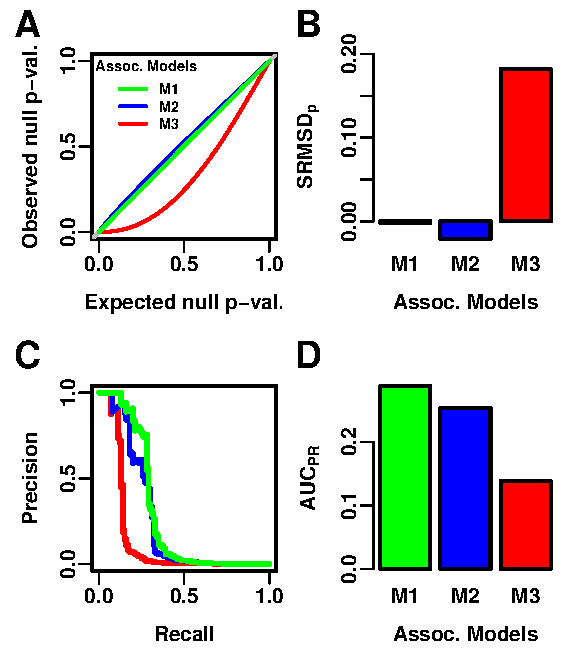
\includegraphics{sim-n1000-k10-f0.1-s0.5-g1/measures-illustration.pdf}
  \caption{
    {\bf Illustration of evaluation measures.}
    Three archetypal models illustrate our complementary measures:
    M1 is ideal, M2 overfits slightly, M3 is naive.
    \textbf{A.}
    QQ plot of p-values of ``null'' (non-causal) loci.
    M1 has desired uniform p-values, M2/M3 are miscalibrated.
    \textbf{B.}
    $\rmsd$ (p-value Signed Root Mean Square Deviation) measures signed distance between observed and expected null p-values (closer to zero is better).
    \textbf{C.}
    Precision and Recall (PR) measure causal locus classification performance (higher is better).
    \textbf{D.}
    $\auc$ (Area Under the PR Curve) reflects power (higher is better).
  }
  \label{fig:measures_illustration}
\end{figure}

% results overview
Both PCA and LMM were evaluated in each replicate dataset including a number of PCs $r$ between 0 and 90 as fixed covariates.
In terms of p-value calibration, for PCA the best number of PCs $r$ (minimizing mean $|\rmsd|$ over replicates) is typically large across all datasets, but much smaller ``min'' $r$ values often performed as well (numbers in parentheses in \cref{tab:human_sum_pcs}).
Most cases had a mean $|\rmsd| < 0.01$ (marked with asterisks in \cref{tab:human_sum_pcs}), whose p-values are effectively calibrated.
However, PCA best and min $r$ values tended to be large on the family simulation and real datasets, and those cases were often miscalibrated.
In contrast, for LMM, $r=0$ (no PCs) was always best, and was always calibrated.
Comparing LMM with $r=0$ to PCA with its best $r$, LMM always had significantly smaller $|\rmsd|$ than PCA or was statistically tied.
%
For $\auc$ and PCA, the best $r$ was always smaller than the best $r$ for $|\rmsd|$, so there is often a tradeoff between calibrated p-values versus classification performance.
For LMM there is no tradeoff, as $r=0$ had $\auc$ not significantly different from the best $r$ in all cases except two (the min $r$ was 2 for both 1000 Genomes simulation with FES trait and 1000 Genomes real dataset with RC trait).
Lastly, LMM with its best $r$ always had significantly greater $\auc$ than PCA with its best $r$ except for one tie (HGDP with RC trait).

\begin{table}[hb!]
  \centering
  %\scriptsize
  \caption{
    \textbf{Overview of PCA and LMM evaluation results}
  }
  \label{tab:human_sum_pcs}
  \csvreader[
  tabular = lc|ccc|ccc,
  separator = tab,
  table head = 
  % header row 1
  \toprule & & \multicolumn{3}{c|}{$|\rmsd|$} & \multicolumn{3}{c}{$\auc$} \\
  % header row 2
  \midrule & & \multicolumn{2}{c}{Best (min\textsuperscript{b}) PCs} & & \multicolumn{2}{c}{Best (min\textsuperscript{b}) PCs} & \\
  % header row 3
  Dataset & {Trait model\textsuperscript{a}} & PCA & LMM & {Best\textsuperscript{c}} & PCA & LMM & {Best\textsuperscript{c}} \\\midrule,
  late after last line = \\\bottomrule
  ]{../data/stats.txt}{}{\csvlinetotablerow}
  \begin{flushleft}
    \textsuperscript{a}FES: Fixed Effect Sizes, RC: Random Coefficients.\\
    \textsuperscript{b}Smallest $r$ (number of PCs) whose distribution ($|\rmsd|$ or $\auc$) was not significantly different (Wilcoxon paired 1-tailed $p > 0.01$) from best $r$ (if any).\\
    \textsuperscript{c}Tie if distributions of best PCA and LMM version did not differ significantly (Wilcoxon paired 1-tailed $p > 0.01$).
    Same result for ``min'' except cases in parentheses.\\
    *$r$ for which mean $|\rmsd| < 0.01$.
  \end{flushleft}
\end{table}

\subsection{Evaluations in admixture simulations}

Now we look more closely at results per dataset.
The complete $\rmsd$ and $\auc$ distributions for the admixture simulations and FES traits are in \cref{fig:rmsd-auc-sim}.
RC traits gave qualitatively similar results (\cref{fig:rmsd-auc-sim-rc}).

In the large admixture simulation, the $\rmsd$ of PCA is largest when $r=0$ (no PCs) and decreases rapidly to near zero at $r=3$, where it stays for up to $r=90$ (\cref{fig:rmsd-auc-sim}A).
Thus, PCA has calibrated p-values for $r \ge 3$, smaller than the theoretical optimum for this simulation of $r = K - 1 = 9$.
In contrast, the $\rmsd$ for LMM starts near zero for $r=0$, but becomes negative as $r$ increases (p-values are conservative).
The $\auc$ distribution of PCA is similarly worst at $r=0$, increases rapidly and peaks at $r = 3$, then decreases slowly for $r > 3$, while the $\auc$ distribution for LMM starts near its maximum at $r=0$ and decreases with $r$.
Although the $\auc$ distributions for LMM and PCA overlap considerably at each $r$, LMM with $r=0$ has significantly greater $\auc$ values than PCA with $r=3$ (\cref{tab:human_sum_pcs}).
However, qualitatively PCA performs nearly as well as LMM in this simulation.

\begin{figure}[bp!]
  \centering
  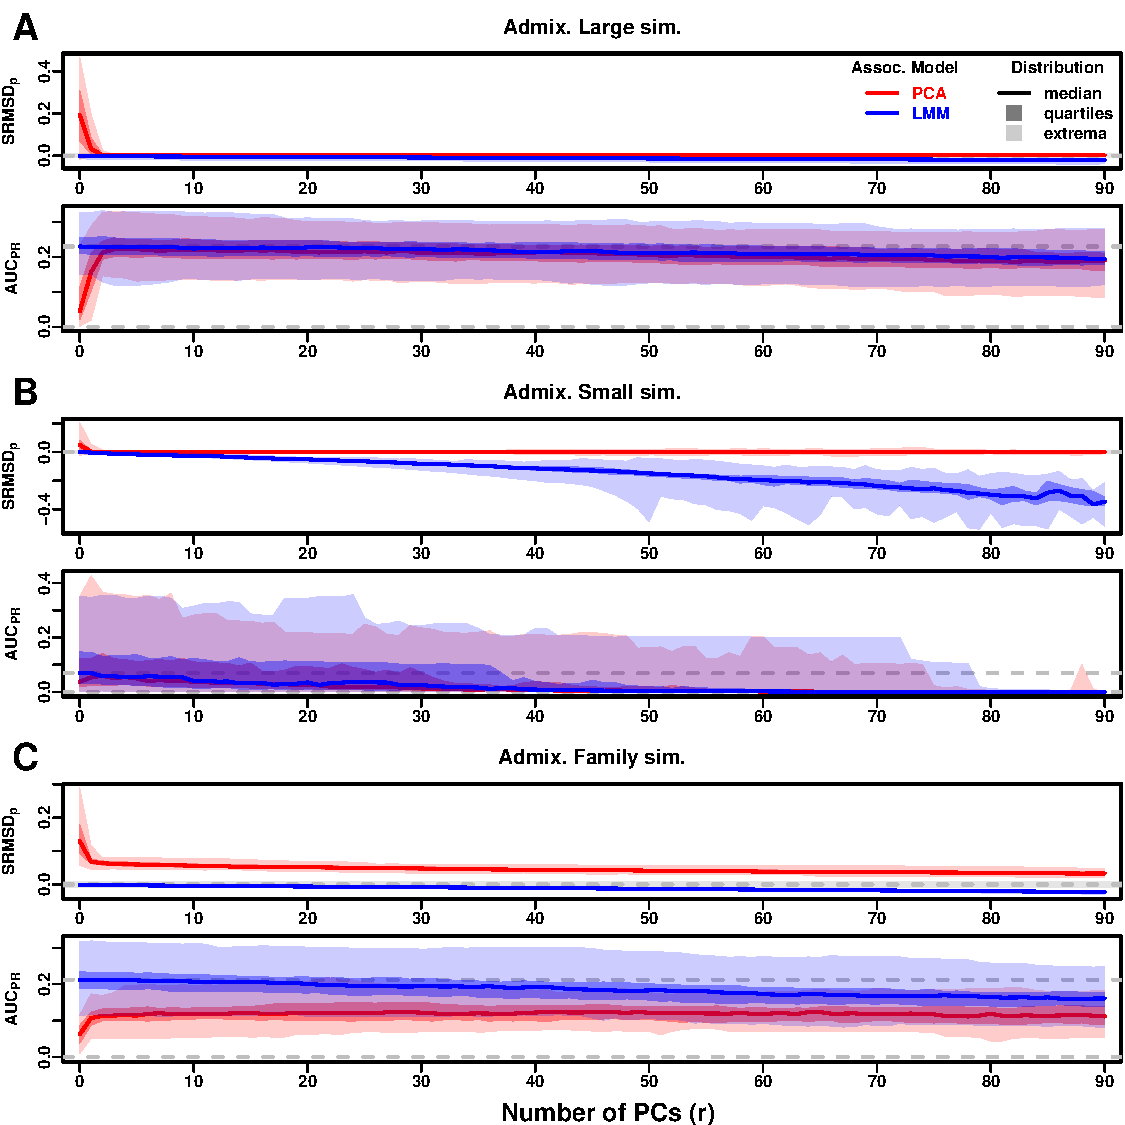
\includegraphics[width=\textwidth,height=\textheight,keepaspectratio]{fes/rmsd-auc-sim.pdf}
  \caption{
    {\small 
      {\bf Evaluations in admixture simulations.}
      Traits simulated from FES model.
      PCA and LMM models have varying number of PCs ($r \in \{0, ..., 90\}$ on x-axis), with the distributions (y-axis) of $\rmsd$ (top subpanel) and $\auc$ (bottom subpanel) for 50 replicates.
      Best performance is zero $\rmsd$ and large $\auc$.
      Zero and maximum median $\auc$ values are marked with horizontal gray dashed lines, and $|\rmsd| < 0.01$ is marked with a light gray area.
      LMM performs best with $r=0$, PCA with various $r$.
      \textbf{A.}
      Large simulation ($n = 1,000$ individuals).
      \textbf{B.}
      Small simulation ($n = 100$) shows overfitting for large $r$.
      \textbf{C.}
      Family simulation ($n = 1,000$) has admixed founders and large numbers of close relatives from a realistic random 20-generation pedigree.
      PCA performs poorly compared to LMM: $\rmsd > 0$ for all $r$ and large $\auc$ gap.
    }
  }
  \label{fig:rmsd-auc-sim}
\end{figure}

The observed robustness to large $r$ led us to consider smaller sample sizes.
A model with large numbers of parameters $r$ should overfit more as $r$ approaches the sample size $n$.
Rather than increase $r$ beyond 90, we reduce individuals to $n = 100$, which is small for typical association studies but may occur in studies of rare diseases, pilot studies, or other constraints.
To compensate for the loss of power due to reducing $n$, we also reduce the number of causal loci (fixed ratio $n / m_1 = 10$), which increases per-locus effect sizes.
We found a large decrease in performance for both models as $r$ increases, and best performance for $r=1$ for PCA and $r=0$ for LMM (\cref{fig:rmsd-auc-sim}B).
Remarkably, LMM attains much larger negative $\rmsd$ values than in our other evaluations.
LMM with $r=0$ is significantly better than PCA ($r=1$ to 4) in both metrics (\cref{tab:human_sum_pcs}), but qualitatively the difference is negligible.

The family simulation adds a 20-generation random family to our large admixture simulation.
Only the last generation is studied for association, which contains numerous siblings, first cousins, etc., with the initial admixture structure preserved by geographically-biased mating.
Our evaluation reveals a sizable gap in both metrics between LMM and PCA across all $r$ (\cref{fig:rmsd-auc-sim}C).
LMM again performs best with $r=0$ and achieves mean $|\rmsd| < 0.01$.
However, PCA does not achieve mean $|\rmsd| < 0.01$ at any $r$, and its best mean $\auc$ is considerably worse than that of LMM.
Thus, LMM is conclusively superior to PCA, and the only calibrated model, when there is family structure.

\subsection{Evaluations in real human genotype datasets}

Next we repeat our evaluations with real human genotype data, which differs from our simulations in allele frequency distributions and more complex population structures with greater differentiation, numerous correlated subpopulations, and potential cryptic family relatedness.

Human Origins has the greatest number and diversity of subpopulations.
The $\rmsd$ and $\auc$ distributions in this dataset and FES traits (\cref{fig:rmsd-auc-real}A) most resemble those from the family simulation (\cref{fig:rmsd-auc-sim}C).
In particular, while LMM with $r=0$ performed optimally (both metrics) and satisfies mean $|\rmsd| < 0.01$, PCA maintained $\rmsd > 0.01$ for all $r$ and its $\auc$ were all considerably smaller than the best $\auc$ of LMM.

\begin{figure}[bp!]
  \centering
  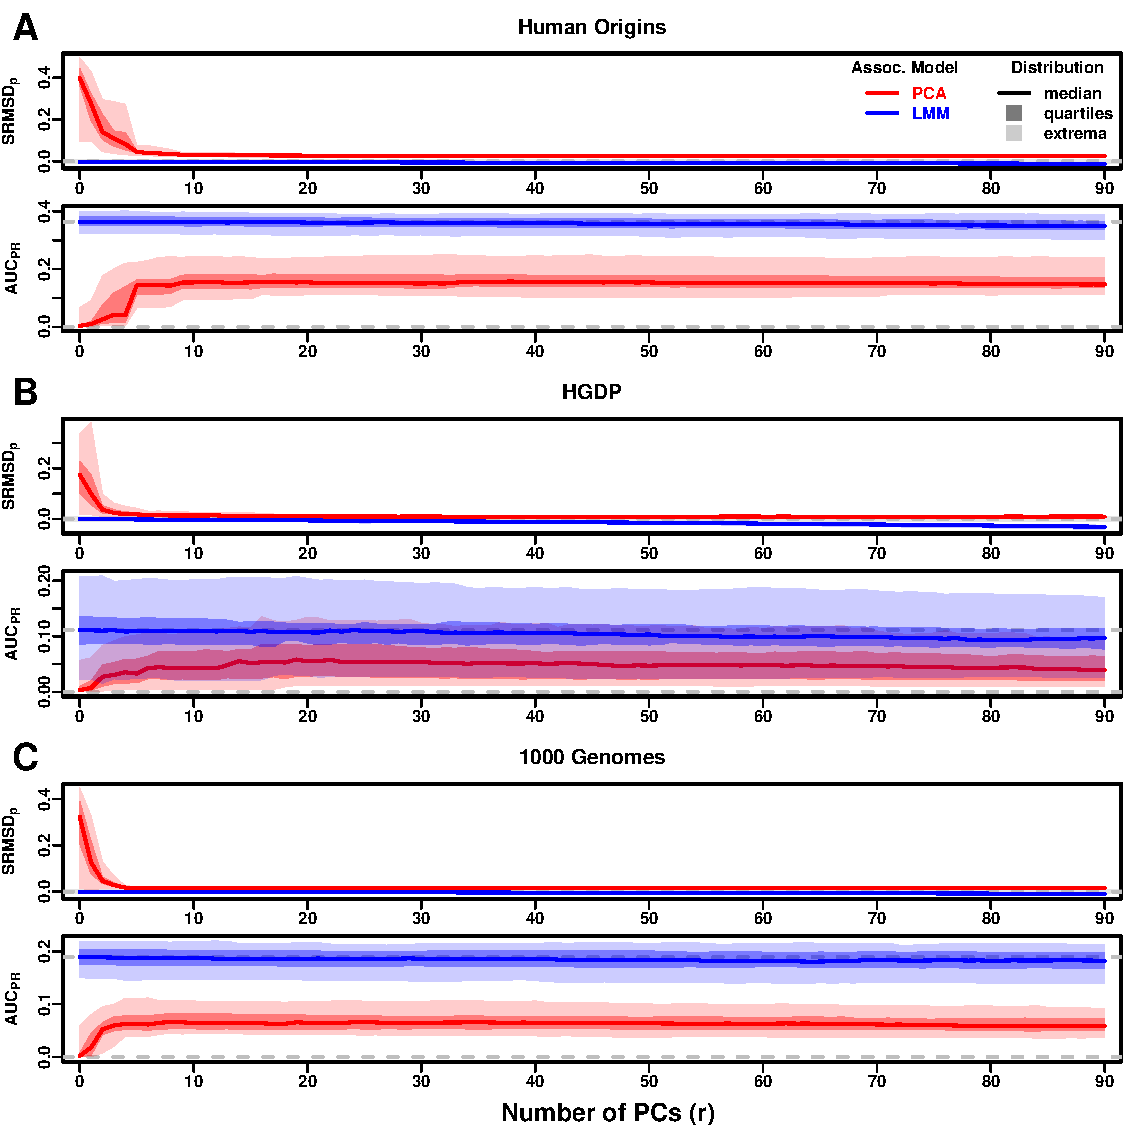
\includegraphics[width=\textwidth,height=\textheight,keepaspectratio]{fes/rmsd-auc-real.pdf}
  \caption{
    {\small 
      {\bf Evaluations in real human genotype datasets.}
      Traits simulated from FES model.
      Same setup as \cref{fig:rmsd-auc-sim}, see that for details.
      These datasets strongly favor LMM with no PCs over PCA, with distributions that most resemble the family simulation.
      \textbf{A.}
      Human Origins.
      \textbf{B.}
      Human Genome Diversity Panel (HGDP).
      \textbf{C.}
      1000 Genomes Project.
    }
  }
  \label{fig:rmsd-auc-real}
\end{figure}

HGDP has the fewest individuals among real datasets, but compared to Human Origins contains more loci and low-frequency variants.
Performance (\cref{fig:rmsd-auc-real}B) was intermediate between the admixture and family simulations.
In particular, here both LMM ($r=0$) and PCA ($r \ge 31$) achieve mean $|\rmsd| < 0.01$ (p-values are calibrated).
However, there is a sizable $\auc$ gap between LMM and PCA.
Maximum $\auc$ values were lowest in HGDP compared to the two other real datasets.

1000 Genomes has the fewest subpopulations but largest number of individuals per subpopulation.
Thus, although this dataset has the simplest subpopulation structure among the real datasets, we find $\rmsd$ and $\auc$ distributions (\cref{fig:rmsd-auc-real}C) that again most resemble our earlier family simulation, with mean $|\rmsd| < 0.01$ for LMM only and large $\auc$ gaps between LMM and PCA.

Our results are qualitatively different for RC traits, which had smaller $\auc$ gaps between LMM and PCA (\cref{fig:rmsd-auc-real-rc}).
Maximum $\auc$ were smaller in RC compared to FES in Human Origins and 1000 Genomes, suggesting lower power for RC traits across association models.
Nevertheless, LMM with $r=0$ was significantly better than PCA for all metrics in the real datasets and RC traits (\cref{tab:human_sum_pcs}).

\subsection{Evaluations in tree simulations fit to human data}

To better understand which features of the real datasets lead to the large differences in performance between LMM and PCA, we carried out tree simulations.
Human subpopulations are related roughly by trees, which induce the strongest correlations and have numerous tips, so we fit trees to each real dataset and tested if data simulated from these complex tree structures could recapitulate our previous results (\cref{fig:kinship}).
These tree simulations also feature non-uniform ancestral allele frequency distributions, which recapitulated some of the skew for smaller minor allele frequencies of the real datasets (\cref{fig:kinship}C).
The $\rmsd$ and $\auc$ distributions for these tree simulations (\cref{fig:rmsd-auc-real-sim}) resembled our admixture simulation more than either the family simulation (\cref{fig:rmsd-auc-sim}) or real data results (\cref{fig:rmsd-auc-real}).
Both LMM with $r=0$ and PCA (various $r$) achieve mean $|\rmsd| < 0.01$ (\cref{tab:human_sum_pcs}).
The $\auc$ distributions of both LMM and PCA track closely as $r$ is varied, although there is a small gap resulting in LMM ($r=0$) besting PCA in all three simulations.
The results are qualitatively similar for RC traits (\cref{fig:rmsd-auc-real-sim-rc,tab:human_sum_pcs}).
Overall, these tree simulations do not recapitulate the large LMM advantage over PCA observed on the real data.

\begin{figure}[bp!]
  \centering
  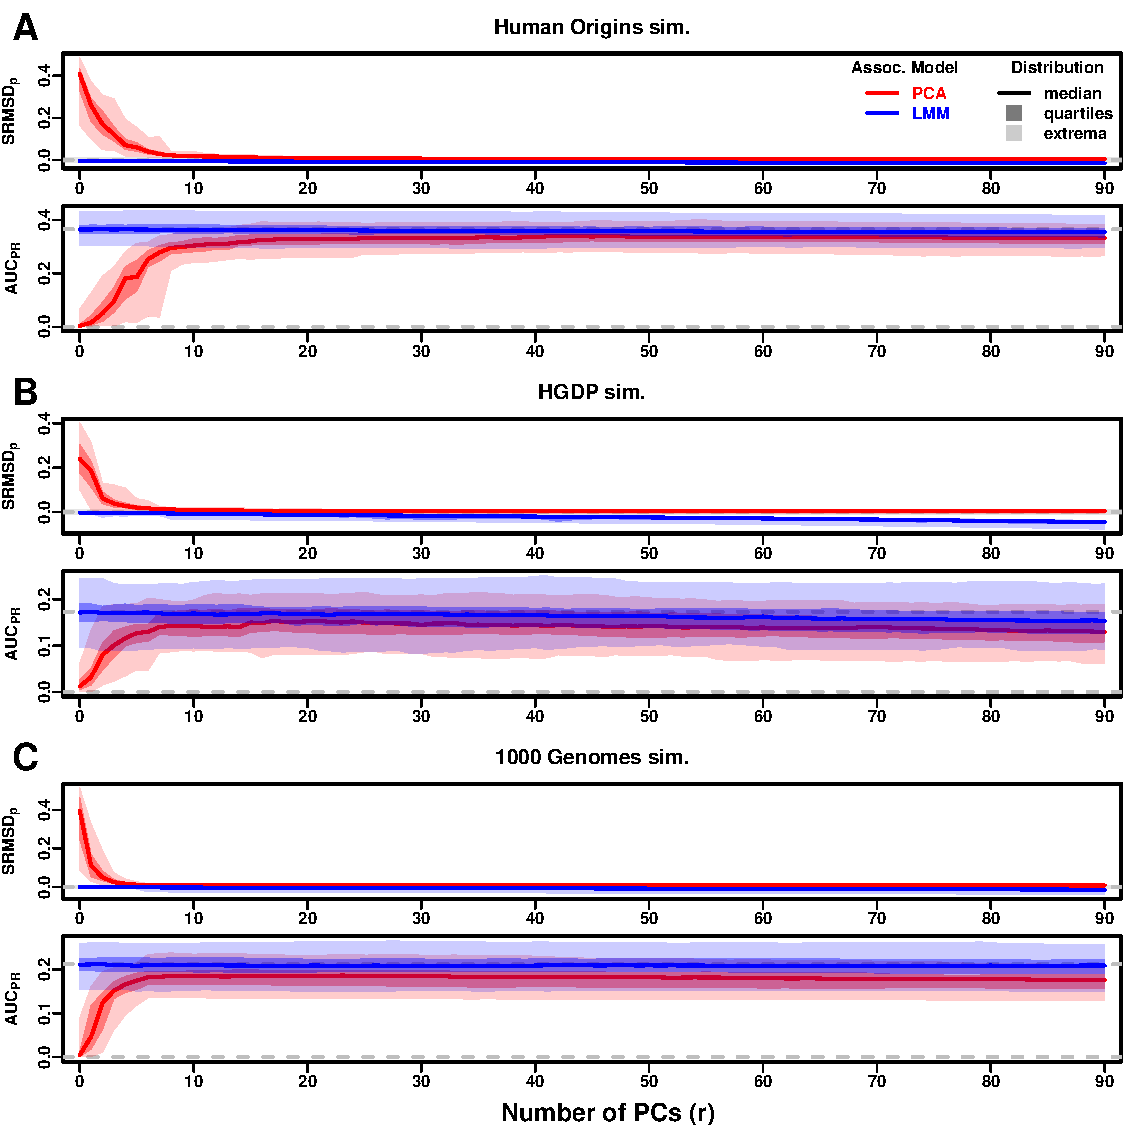
\includegraphics[width=\textwidth,height=\textheight,keepaspectratio]{fes/rmsd-auc-real-sim.pdf}
  \caption{
    {\small 
      {\bf Evaluations in tree simulations fit to human data.}
      Traits simulated from FES model.
      Same setup as \cref{fig:rmsd-auc-sim}, see that for details.
      These tree simulations, which exclude family structure by design, do not explain the large gaps in LMM-PCA performance observed in the real data.
      \textbf{A.}
      Human Origins tree simulation.
      \textbf{B.}
      Human Genome Diversity Panel (HGDP) tree simulation.
      \textbf{C.}
      1000 Genomes Project tree simulation.
    }
  }
  \label{fig:rmsd-auc-real-sim}
\end{figure}

\subsection{Numerous distant relatives explain poor PCA performance in real data}

In principle, PCA performance should be determined by the dimensionality of relatedness, since PCA is a low-dimensional model whereas LMM can model high-dimensional relatedness without overfitting.
We used the Tracy-Widom test \citep{patterson_population_2006} with $p < 0.01$ to estimate dimensionality as the number of significant PCs (\cref{fig:eigen}A).
The true dimensionality of our simulations is slightly underestimated (\cref{tab:human_sum}), but we confirm that the family simulation has the greatest dimensionality, and real datasets have greater estimates than their respective tree simulations, which confirms our hypothesis to some extent.
However, estimated dimensionalities do not separate real datasets from tree simulations, as required to predict the observed PCA performance.
Moreover, the HGDP and 1000 Genomes dimensionality estimates are 46 and 61, respectively, yet PCA performed poorly for all $r \le 90$ numbers of PCs (\cref{fig:rmsd-auc-real}).
The top eigenvalue explained a proportion of variance proportional to \Fst (\cref{tab:human_sum}), but the rest of the top 10 eigenvalues show no clear differences between datasets, except the small simulation had larger variances explained per eigenvalue (expected since it has fewer eigenvalues; \cref{fig:eigen}C).
Comparing cumulative variance explained versus rank fraction across all eigenvalues, all datasets increase from their starting point almost linearly until they reach 1, except the family simulation has much greater variance explained by mid-rank eigenvalues (\cref{fig:eigen}B).
Overall, there is no separation between real datasets (where PCA performed poorly) and tree simulations (where PCA performed relatively well) in terms of their eigenvalues or dimensionality estimates.

Local kinship, which is recent relatedness due to family structure excluding population structure, is the presumed cause of the LMM to PCA performance gap observed in real datasets but not their tree simulation counterparts.
Instead of inferring local kinship through increased dimensionality, as attempted in the last section, here we measure it directly using the KING-robust estimator \citep{manichaikul_robust_2010}.
We observe more large local kinship in the real datasets and the family simulation compared to the other simulations (\cref{fig:king}).
However, for real data this distribution depends on the subpopulation structure, since locally related pairs are most likely in the same subpopulation.
Therefore, the only comparable curve to each real dataset is their corresponding tree simulation, which matches subpopulation structure.
In all real datasets we identified highly related individual pairs with kinship above the 4th degree relative threshold of 0.022 \citep{manichaikul_robust_2010, conomos_model-free_2016}.
However, these highly related pairs are vastly outnumbered by more distant pairs with evident non-zero local kinship as compared to the extreme tree simulation values.

\begin{figure}[bp!]
  \centering
  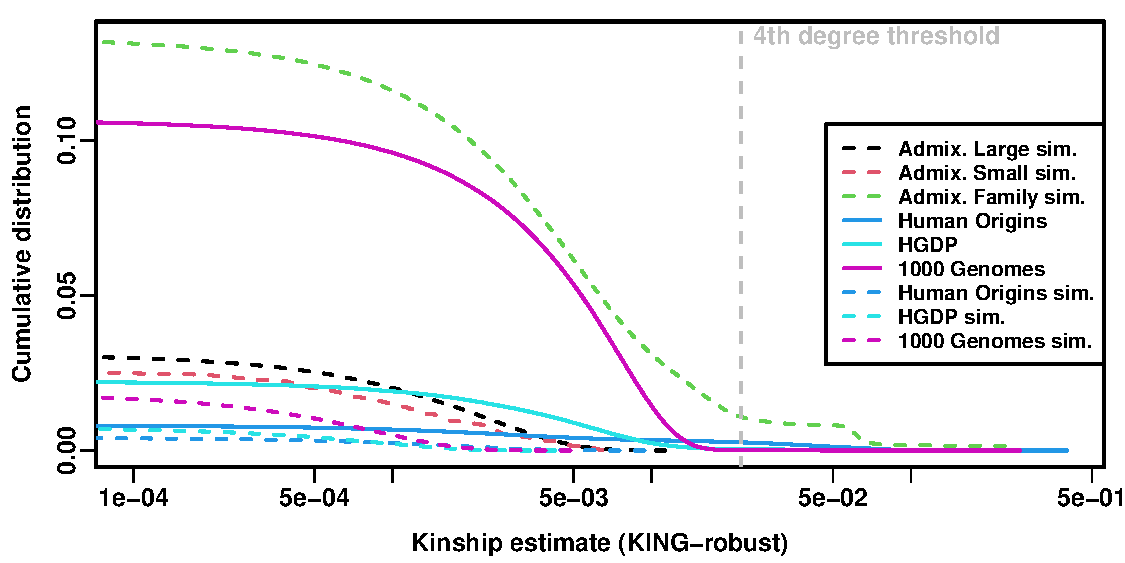
\includegraphics[width=\textwidth]{king_log-x.pdf}
  \caption{
    {\bf Local kinship distribution.}
    Curves are complementary cumulative distribution of lower triangular kinship matrix (self kinship excluded) from KING-robust estimator.
    Note log x-axis; negative estimates are counted but not shown.
    Most values are below 4th degree relative threshold.
    Each real dataset has a greater cumulative than its tree simulations.
  }
  \label{fig:king}
\end{figure}

To try to improve PCA performance, we followed the standard practice of removing 4th degree relatives, which reduced sample sizes between 5\% and 10\% (\cref{tab:king_cutoff}).
Only $r=0$ for LMM and $r=20$ for PCA were tested, as these performed well in our earlier evaluation, and only FES traits were tested because they previously displayed the large PCA-LMM performance gap.
LMM significantly outperforms PCA in all these cases (Wilcoxon paired 1-tailed $p < 0.01$; \cref{fig:king_cutoff}).
Notably, PCA still had miscalibrated p-values in Human Origins and 1000 Genomes ($|\rmsd| > 0.01$).
Otherwise, $\auc$ and $\rmsd$ ranges were similar here as in our earlier evaluation.
Therefore, the removal of the small number of highly related individual pairs had a negligible effect in PCA performance, so the larger number of more distantly related pairs explain the poor PCA performance in the real datasets.

\begin{figure}[bp!]
  \centering
  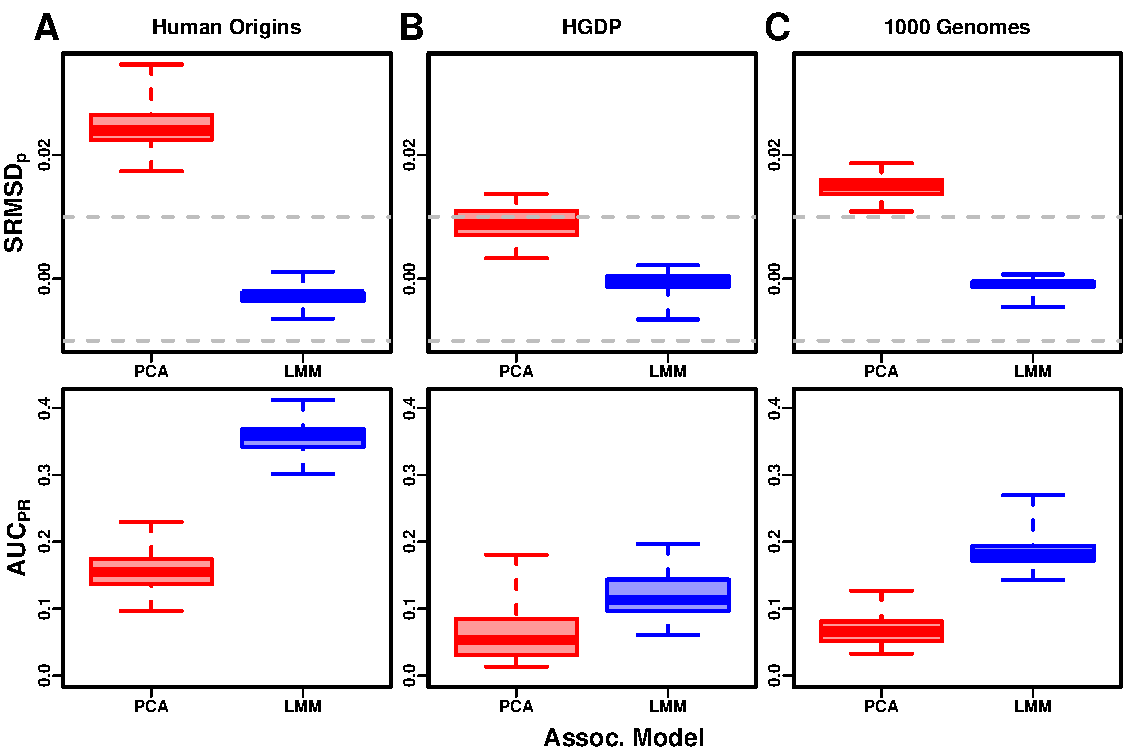
\includegraphics[width=\textwidth]{fes/rmsd-auc_king-cutoff-4.pdf}
  \caption{
    {\bf LMM and PCA performance in real datasets excluding 4th degree relatives.}
    LMM had $r=0$ PCs and PCA had $r=20$.
    FES traits only.
    Each dataset is a column, rows are metrics.
    First row has $|\rmsd| < 0.01$ band marked as gray area.
  }
  \label{fig:king_cutoff}
\end{figure}


\section{Discussion}

% LMM r=0 best, r>0 not good
Our evaluations conclusively determined that LMM without PCs performs better than PCA (for any number of PCs) across all scenarios, including all real and simulated genotypes and two trait simulation models.
Although the addition of a few PCs to LMM does not greatly hurt its performance (except for small sample sizes), they generally did not improve it either (\cref{tab:human_sum_pcs}), which agrees with previous observations \citep{liu_controlling_2011} but contradicts others \citep{zhao_arabidopsis_2007, price_new_2010}.
Our findings make sense since PCs are the eigenvectors of the same kinship matrix that parametrizes random effects, so including both is redundant.

% unusually differentiated markers
Previous studies found that PCA was better calibrated than LMM for unusually differentiated markers \citep{price_new_2010, wu_comparison_2011, yang_advantages_2014}, which as simulated were an artificial scenario not based on a population genetics model, and are otherwise believed to be unusual \citep{sul_mixed_2013, price_response_2013}.
Our evaluations on real human data, which contain such loci in relevant proportions if they exist, do not replicate that result.
Cryptic relatedness strongly favors LMM, an advantage that probably outweighs this potential PCA benefit in real data.

% PCA two extremes
Relative to LMM, the behavior of PCA fell between two extremes.
When PCA performed well, there was a small number of PCs with both calibrated p-values and $\auc$ near that of LMM without PCs.
Conversely, PCA performed poorly when no number of PCs had either calibrated p-values or acceptably large $\auc$.
There were no PCA cases where high numbers of PCs optimized an acceptable $\auc$, or miscalibrated p-values but high $\auc$.
PCA performed well in the admixture simulations (without families, both trait models), real human genotypes with RC traits, and, to a lesser extent, the tree simulations (both trait models).
Conversely, PCA performed poorly in the admixed family simulation (both trait models) and the real human genotypes with FES traits.

% PCA vs dimensionality, local kinship
PCA assumes that genetic relatedness is low-dimensional, whereas LMM can handle high-dimensional relatedness.
Thus, PCA performs well in the admixture simulation, which is explicitly low-dimensional (see Models and Methods), and our tree simulations, which had few nodes with long branches so a low-dimensional approximation suffices.
Conversely, PCA performs poorly under family structure because its kinship matrix is high-dimensional (\cref{fig:eigen}).
However, estimating the dimensionality of real datasets is challenging because estimated eigenvalues have biased distributions.
Dimensionality estimated using the Tracy-Widom test \citep{patterson_population_2006} did not fully predict the datasets that PCA performs well on.
In contrast, estimated local kinship finds considerable cryptic relatedness in all real human datasets and better explains why PCA performs poorly there.
The trait model also influences the relative performance of PCA, so genotype-only parameters (eigenvalues or local kinship) alone do not tell the full story.

% evidence that distant relatives are cause for poor PCA performance
PCA is at best underpowered relative to LMMs, and at worst miscalibrated regardless of the numbers of PCs included, in real human genotype tests.
Among our simulations, such poor performance occurred only in the admixed family.
Local kinship estimates reveal considerable family relatedness in the real datasets absent in the corresponding tree simulations.
Admixture is also absent in our tree simulations, but our simulations and theory show that admixture is handled well by PCA.
Hundreds of close relative pairs have been identified in 1000 Genomes \citep{gazal_high_2015, al-khudhair_inference_2015, fedorova_atlas_2016, schlauch_identification_2017}, but their removal does not improve PCA performance sufficiently in our tests, so the larger number of more distantly related pairs are PCA's most serious obstacle in practice.
Distant relatives are expected to be numerous in any large human dataset \citep{henn_cryptic_2012, shchur_number_2018}.
Our FES trait tests show that cryptic relatedness is more challenging when rarer variants have larger coefficients.
Overall, the high dimensionality induced by cryptic relatedness is the key challenge for PCA association in modern datasets that is readily overcome by LMM.

% high r robustness in PCA but not this LMM
Our tests also found PCA robust to large numbers of PCs, far beyond the optimal choice, agreeing with previous anecdotal observations \citep{price_principal_2006, kang_variance_2010}, in contrast to using too few PCs for which there is a large performance penalty.
The exception was the small sample size simulation, where only small numbers of PCs performed well.
In contrast, LMM is simpler since there is no need to choose the number of PCs.
However, an LMM with a large number of covariates may have conservative p-values (as observed for LMM with large numbers of PCs), a weakness of the score test used by the LMM we evaluated that may be overcome with other statistical tests.
Simulations or post hoc evaluations remain crucial for ensuring that statistics are calibrated.

% Q vs CC traits
The largest limitation of our work is that we only considered quantitative traits.
We noted that previous evaluations involving case-control traits tended to report PCA-LMM ties or mixed results, an observation potentially confounded by the use of low-dimensional simulations without family relatedness (\cref{tab:lit}).
An additional concern is case-control ascertainment bias, which appears to affect LMMs more severely, although recent work appears to solve this problem \citep{yang_advantages_2014, zhou_efficiently_2018}.
Future evaluations should aim to include our simulations and real datasets, to ensure that previous results were not biased in favor of PCA by employing unrealistic low-dimensional genotype simulations, or by not simulating large coefficients for rare variants expected for diseases by various selection models.

% closing
Overall, our results lead us to recommend LMM over PCA for association studies in general.
Although PCA offer flexibility and speed compared to LMM, additional work is required to ensure that PCA is adequate, including removal of close relatives (lowering sample size and wasting resources) followed by simulations or other evaluations of statistics, and even then PCA may perform poorly in terms of both type I error control and power.
The large numbers of distant relatives expected of any real dataset all but ensures that PCA will perform poorly compared to LMM.
Our findings also suggest that related applications such as polygenic models may enjoy gains in power and accuracy by employing an LMM instead of PCA to model relatedness \citep{rakitsch_lasso_2013,qian_fast_2020}.
PCA remains indispensable across population genetics, from visualizing population structure and performing quality control to its deep connection to admixture models, but the time has come to limit its use in association testing in favor of LMM or other, richer models capable of modeling all forms of relatedness.

%%%TODOTODOTODO

\section{Appendices}

\subsection{Appendix A: Fitting ancestral allele frequency distribution to real data}

We calculated \pith distributions of each real dataset.
However, differentiation increases the variance of these sample \pith relative to the true \pit \citep{ochoa_estimating_2021}.
We present a new algorithm for constructing an ``undifferentiated'' distribution based on the input data but with the lower variance of the true ancestral distribution.
Suppose the \pit distribution over loci $i$ satisfies $\E \left[ \pit \right] = \frac{1}{2}$ and $\Var \left( \pit \right) = V^T$.
The sample allele frequency \pith, conditioned on \pit, satisfies
$$
\E \left[ \pith \middle| \pit \right]
=
\pit
, \quad\quad
\Var \left( \pith \middle| \pit \right)
=
\pit \left( 1 - \pit \right) \bar{\varphi}^T
,
$$
where $\bar{\varphi}^T = \frac{1}{n^2} \sum_{j=1}^n \sum_{k=1}^n \kt$ is the mean kinship over all individual \citep{ochoa_estimating_2021}.
The unconditional moments of \pith follow from the laws of total expectation and variance: 
$
\E \left[ \pith \right]
% =
% \E \left[ \E \left[ \pith \middle| \pit \right] \right]
=
\frac{1}{2}
$
and
\begin{equation*}
  W^T
  =
  \Var \left( \pith \right)
  % &=
  %   \E \left[ \Var \left( \pith \middle| \pit \right) \right ]
  %   + \Var \left( \E \left[ \pith \middle| \pit \right] \right)
  % \\
  % &=
  %   \E \left[ \pit \left( 1 - \pit \right) \bar{\varphi}^T \right]
  %   + \Var \left( \pit \right)
  % \\
  % &=
  %   \bar{\varphi}^T \E \left[ \pit \right] \left( 1 - \E \left[ \pit \right] \right)
  %   + \left( 1 - \bar{\varphi}^T \right) \Var \left( \pit \right)
  % \\
  =
  \bar{\varphi}^T \frac{1}{4}
  + \left( 1 - \bar{\varphi}^T \right) V^T
  .
\end{equation*}
Since $V^T \le \frac{1}{4}$ and $\bar{\varphi}^T \ge 0$, then $W^T \ge V^T$.
Thus, the goal is to construct a new distribution with the original, lower variance of
\begin{equation}
  \label{eq:var_undiff}
  V^T
  =
  \frac{ W^T - \frac{1}{4} \bar{\varphi}^T }{ 1 - \bar{\varphi}^T }
  .
\end{equation}
We use the unbiased estimator
$
\hat{W}^T
=
\frac{1}{m} \sum_{i=1}^m \left( \pith - \frac{1}{2} \right)^2
,
$
while $\bar{\varphi}^T$ is calculated from the tree parameters: the subpopulation coancestry matrix (\cref{eq:coanc_tree_additive}), expanded from subpopulations to individuals, the diagonal converted to kinship (reversing \cref{eq:kinship_to_coanc}), and the matrix averaged.
However, since our model ignores the MAF filters imposed in our simulations, $\bar{\varphi}^T$ was adjusted.
For Human Origins the true model $\bar{\varphi}^T$ of 0.143 was used.
For 1000 Genomes and HGDP the true $\bar{\varphi}^T$ are 0.126 and 0.124, respectively, but 0.4 for both produced a better fit.

Lastly, we construct new allele frequencies,
$$
p' = w \pith + ( 1 - w ) q,
$$
by a weighted average of \pith and $q \in (0, 1)$ drawn independently from a different distribution.
$\E[q] = \frac{1}{2}$ is required to have $\E \left[ p' \right] = \frac{1}{2}$.
The resulting variance is
$$
\Var(p')
=
w^2 W^T + (1-w)^2 \Var(q)
,
$$
which we equate to the desired $V^T$ (\cref{eq:var_undiff}) and solve for $w$.
For simplicity, we also set $\Var(q) = V^T$, which is achieved with:
$$
q \sim \text{Beta} \left( \frac{1}{2} \left( \frac{1}{ 4 V^T } - 1 \right), \frac{1}{2} \left( \frac{1}{ 4 V^T } - 1 \right) \right)
.
$$
Although $w=0$ yields $\Var(p') = V^T$, we use the second root of the quadratic equation to use \pith:
$$
w = \frac{ 2 V^T }{ W^T + V^T }.
$$



\subsection{Appendix B: comparisons between $\rmsd$, $\auc$, and evaluation measures from the literature}

\subsubsection{The inflation factor $\lambda$}

Test statistic inflation has been used to measure model calibration \citep{astle_population_2009, price_new_2010}.
The inflation factor $\lambda$ is defined as the median $\chi^2$ association statistic divided by theoretical median under the null hypothesis \citep{devlin_genomic_1999}.
To compare p-values from non-$\chi^2$ tests (such as t-statistics), $\lambda$ can be calculated from p-values using
$$
\lambda
=
\frac{
  F^{-1} \left( 1 - p_\text{median} \right)
}{
  F^{-1} \left( 1 - u_\text{median} \right)
}
,
$$
where $p_\text{median}$ is the median observed p-value (including causal loci),
$u_\text{median} = \frac{1}{2}$ is its null expectation,
and $F$ is the $\chi^2$ cumulative density function ($F^{-1}$ is the quantile function).

To compare $\lambda$ and $\rmsd$ directly, for simplicity assume that all p-values are null.
In this case, calibrated p-values give $\lambda = 1$ and $\rmsd = 0$.
However, non-uniform p-values with the expected median, such as from genomic control \citep{devlin_genomic_1999}, result in $\lambda = 1$, but $\rmsd \ne 0$ except for uniform p-values, a key flaw of $\lambda$ that $\rmsd$ overcomes.
Inflated statistics (anti-conservative p-values) give $\lambda > 1$ and $\rmsd > 0$.
Deflated statistics (conservative p-values) give $\lambda < 1$ and $\rmsd < 0$.
Thus, $\lambda \ne 1$ always implies $\rmsd \ne 0$ (where $\lambda - 1$ and $\rmsd$ have the same sign), but not the other way around.
Overall, $\lambda$ depends only on the median p-value, while $\rmsd$ uses the complete distribution.
However, $\rmsd$ requires knowing which loci are null, so unlike $\lambda$ it is only applicable to simulated traits.

\subsubsection{Empirical comparison of $\rmsd$ and $\lambda$}

There is a near one-to-one correspondence between $\lambda$ and $\rmsd$ in our data (\cref{fig:rmsd_lambda}).
PCA tended to be inflated ($\lambda > 1$ and $\rmsd > 0$) whereas LMM tended to be deflated ($\lambda < 1$ and $\rmsd < 0$), otherwise the data for both models fall on the same contiguous curve.
We fit a sigmoidal function to this data,
\begin{equation}
  \label{eq:rmsd_lambda_sigmoidal}
  \rmsd( \lambda ) = a \frac{ \lambda^b - 1 }{ \lambda^b + 1 },
\end{equation}
% inverse:
% lambda <- ( ( a + rmsd ) / ( a - rmsd ) )^(1/b)
which for $a,b > 0$ satisfies $\rmsd( \lambda = 1 ) = 0$ and reflects $\log( \lambda )$ about zero ($\lambda = 1$):
$$
\rmsd( \log( \lambda ) = -x ) = - \rmsd( \log( \lambda ) = x ).
$$
% \rmsd
% = a \frac{ e^{-bx} - 1 }{ e^{-bx} + 1 }
% = a \frac{ 1 - e^{bx} }{ 1 + e^{bx} }
We fit this model to $\lambda > 1$ only since it was less noisy and of greater interest, and obtained the curve shown in \cref{fig:rmsd_lambda} with $a = 0.566$ and $b = 0.616$.
% Using this model, we also produced a log-linear approximation based on its Taylor series with respect to $x = \log( \lambda )$ about $x=0$, resulting in
% \begin{equation}
%   \label{eq:rmsd_lambda_log_linear}
%   \rmsd( \lambda ) \approx \frac{a b}{2} \log( \lambda ).
% \end{equation}
% % inverse:
% % lambda <- exp( 2 * rmsd / ( a * b ) )
The value $\lambda = 1.05$, a common threshold for benign inflation \citep{price_new_2010}, corresponds to $\rmsd = 0.0085$ according to \cref{eq:rmsd_lambda_sigmoidal}.
Conversely, $\rmsd = 0.01$, serving as a simpler rule of thumb, corresponds to $\lambda = 1.06$.

\subsubsection{Type I error rate}

The type I error rate is the proportion of null p-values with $p \le t$.
Calibrated p-values have type I error rate near $t$, which may be evaluated with a binomial test.
This measure may give different results for different $t$, for example be significantly miscalibrated only for large $t$ (due to lack of power for smaller $t$).
In contrast, $\rmsd = 0$ guarantees calibrated type I error rates at all $t$, while large $|\rmsd|$ indicates incorrect type I errors for a range of $t$.

\subsubsection{Statistical power and comparison to $\auc$}

Power is the probability that a test is declared significant when the alternative hypothesis $H_1$ holds.
At a p-value threshold $t$, power equals
$$
F(t) = \Pr( p < t | H_1 ).
$$
$F(t)$ is a cumulative function, so it is monotonically increasing and has an inverse.
Like type I error control, power may rank models differently depending on $t$.

Power is not meaningful when p-values are not calibrated.
To establish a clear connection to $\auc$, assume calibrated (uniform) null p-values: $\Pr( p < t | H_0 ) = t$.
TPs, FPs, and FNs at $t$ are
\begin{align*}
  \text{TP}(t)
  &=
    m \pi_1 F(t)
    , \\
  \text{FP}(t)
  &=
    m \pi_0 t
    , \\
  \text{FN}(t)
  &=
    m \pi_1 ( 1 - F(t) )
    ,
\end{align*}
where $\pi_0 = \Pr( H_0 )$ is the proportion of null cases and $\pi_1 = 1 - \pi_0$ of alternative cases.
Therefore, 
\begin{align*}
  \text{Precision}(t)
  &=
    \frac{ \pi_1 F(t) }{ \pi_1 F(t) + \pi_0 t }
    , \\
  \text{Recall}(t)
  &=
    F(t)
    .
\end{align*}
Noting that $t = F^{-1}( \text{Recall} )$, precision can be written as a function of recall, the power function, and constants:
\begin{align*}
  \text{Precision}( \text{Recall} )
  &=
    \frac{ \pi_1 \text{Recall} }{ \pi_1 \text{Recall} + \pi_0 F^{-1}( \text{Recall} ) }
    .
\end{align*}
This last form leads most clearly to
$
\auc
=
\int_0^1 \text{Precision}( \text{Recall} ) d \text{Recall}
$
.

Lastly, consider a simple yet common case in which model $A$ is uniformly more powerful than model $B$: $F_A(t) > F_B(t)$ for every $t$.
Therefore $F_A^{-1}( \text{Recall} ) < F_B^{-1}( \text{Recall} )$ for every recall value.
This ensures that the precision of $A$ is greater than that of $B$ at every recall value, so $\auc$ is greater for $A$ than $B$.
Thus, $\auc$ ranks calibrated models according to power.


\section*{Declaration of interests}
The authors declare no competing interests.

\section*{Acknowledgments}
The 1000 Genomes data were generated at the New York Genome Center with funds provided by NHGRI Grant 3UM1HG008901-03S1.

\section*{Web resources}
plink2, \url{https://www.cog-genomics.org/plink/2.0/}\\
GCTA, \url{https://yanglab.westlake.edu.cn/software/gcta/}\\
Eigensoft, \url{https://github.com/DReichLab/EIG}\\g
bnpsd, \url{https://cran.r-project.org/package=bnpsd}\\
simfam, \url{https://cran.r-project.org/package=simfam}\\
simtrait, \url{https://cran.r-project.org/package=simtrait}\\
genio, \url{https://cran.r-project.org/package=genio}\\
popkin, \url{https://cran.r-project.org/package=popkin}\\
ape, \url{https://cran.r-project.org/package=ape}\\
nnls, \url{https://cran.r-project.org/package=nnls}\\
PRROC, \url{https://cran.r-project.org/package=PRROC}\\
BEDMatrix, \url{https://cran.r-project.org/package=BEDMatrix}

\section*{Data and code availability}
The data and code generated during this study are available on GitHub at \url{https://github.com/OchoaLab/pca-assoc-paper}.
The public subset of Human Origins is available on the Reich Lab website at \url{https://reich.hms.harvard.edu/datasets}; non-public samples have to be requested from David Reich.
The WGS version of HGDP was downloaded from the Wellcome Sanger Institute FTP site at \url{ftp://ngs.sanger.ac.uk/production/hgdp/hgdp_wgs.20190516/}.
The high-coverage version of the 1000 Genomes Project was downloaded from \url{ftp://ftp.1000genomes.ebi.ac.uk/vol1/ftp/data_collections/1000G_2504_high_coverage/working/20190425_NYGC_GATK/}.



\printbibliography

%%%%%%%%%%%%%%%%%%%%%%%%%%%%%%%%% 
%%% SUPPLEMENTARY INFORMATION %%%
%%%%%%%%%%%%%%%%%%%%%%%%%%%%%%%%%

\clearpage

\beginsupplement

\section{Supplementary figures}

\begin{figure}[hp!]
  \centering
  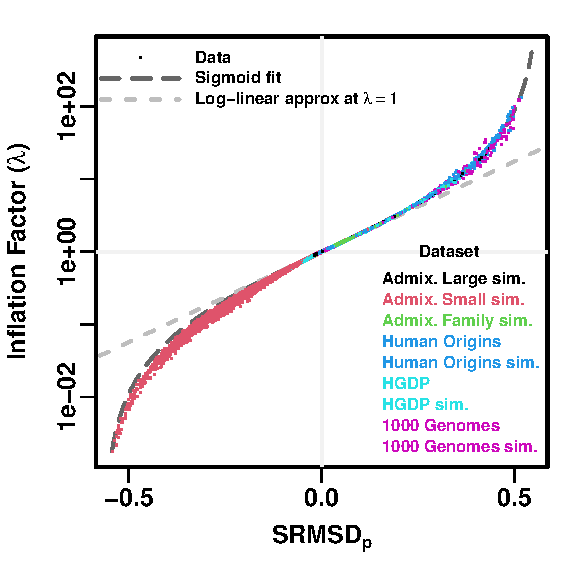
\includegraphics{sum-rmsd-vs-lambda.pdf}
  \caption{
    {\bf Comparison between $\rmsd$ and inflation factor.}
    Each point is a pair of statistics for one replicate, one association model (PCA or LMM with some number of PCs $r$), one trait model (FES vs RC), and one dataset (color coded by dataset).
    Note log y-axis ($\lambda$).
    The sigmoidal curve in \cref{eq:rmsd_lambda_sigmoidal} is fit to the data.
  }
  \label{fig:rmsd_lambda}
\end{figure}

\begin{figure}[hp!]
  \centering
  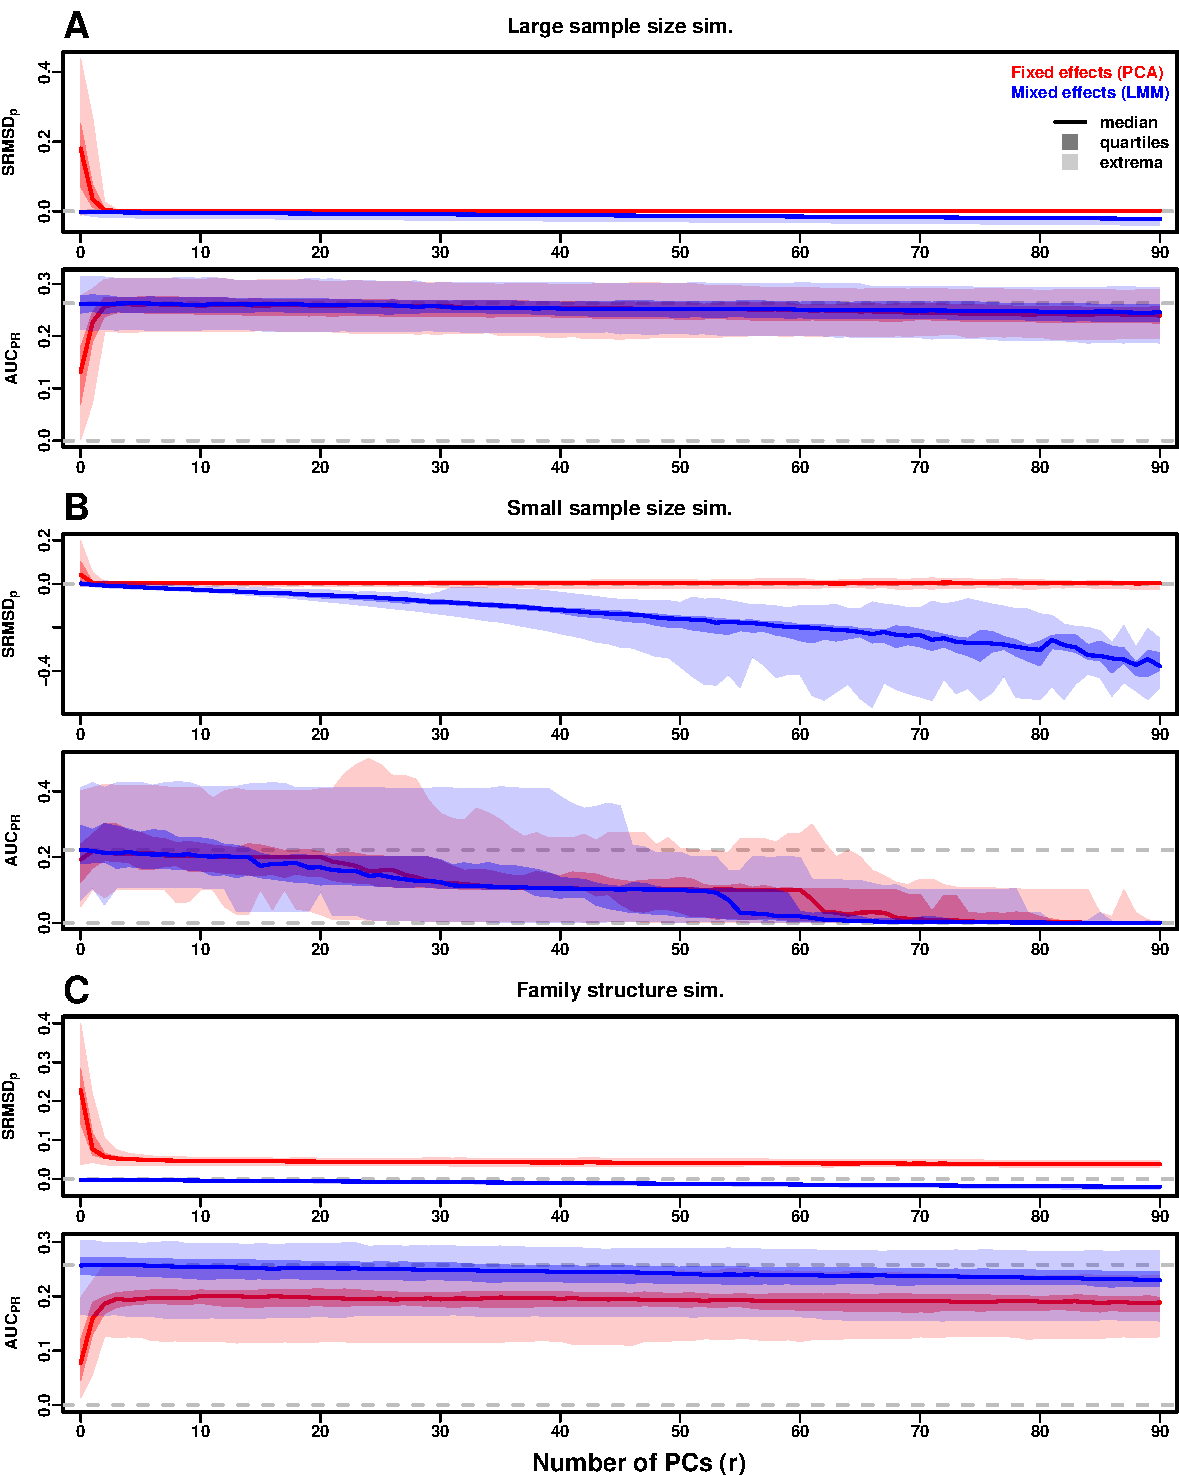
\includegraphics[width=\textwidth,height=\textheight,keepaspectratio]{rmsd-auc-sim.pdf}
  \caption{
    {\small 
      {\bf Evaluations in admixture simulations.}
      Traits simulated from RC model, otherwise the same as \cref{fig:rmsd-auc-sim}.
    }
  }
  \label{fig:rmsd-auc-sim-rc}
\end{figure}

\begin{figure}[hp!]
  \centering
  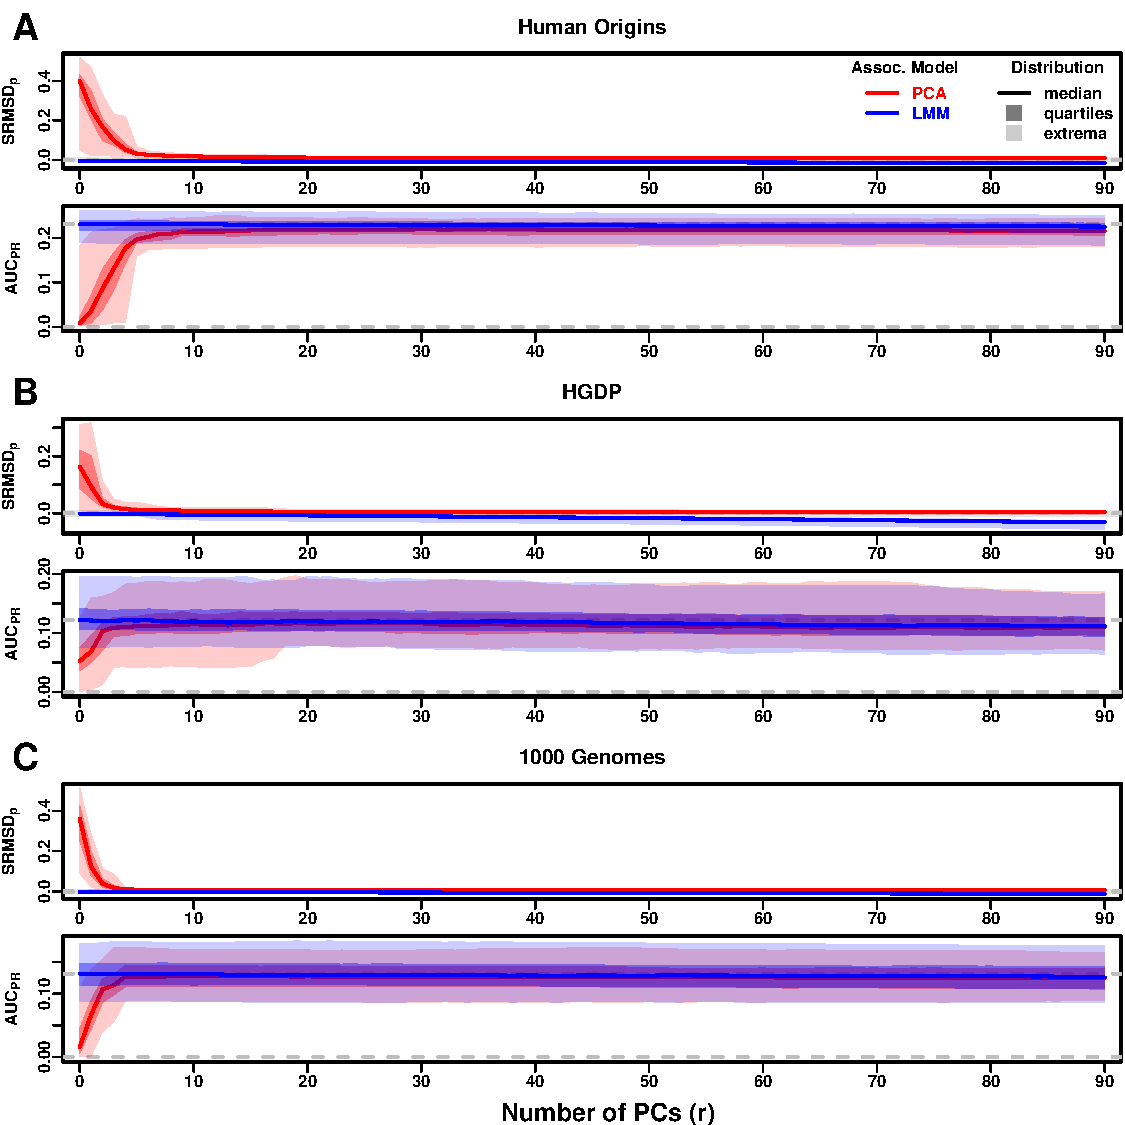
\includegraphics[width=\textwidth,height=\textheight,keepaspectratio]{rmsd-auc-real.pdf}
  \caption{
    {\small 
      {\bf Evaluations in real human genotype datasets.}
      Traits simulated from RC model, otherwise the same as \cref{fig:rmsd-auc-real}.
    }
  }
  \label{fig:rmsd-auc-real-rc}
\end{figure}

\begin{figure}[hp!]
  \centering
  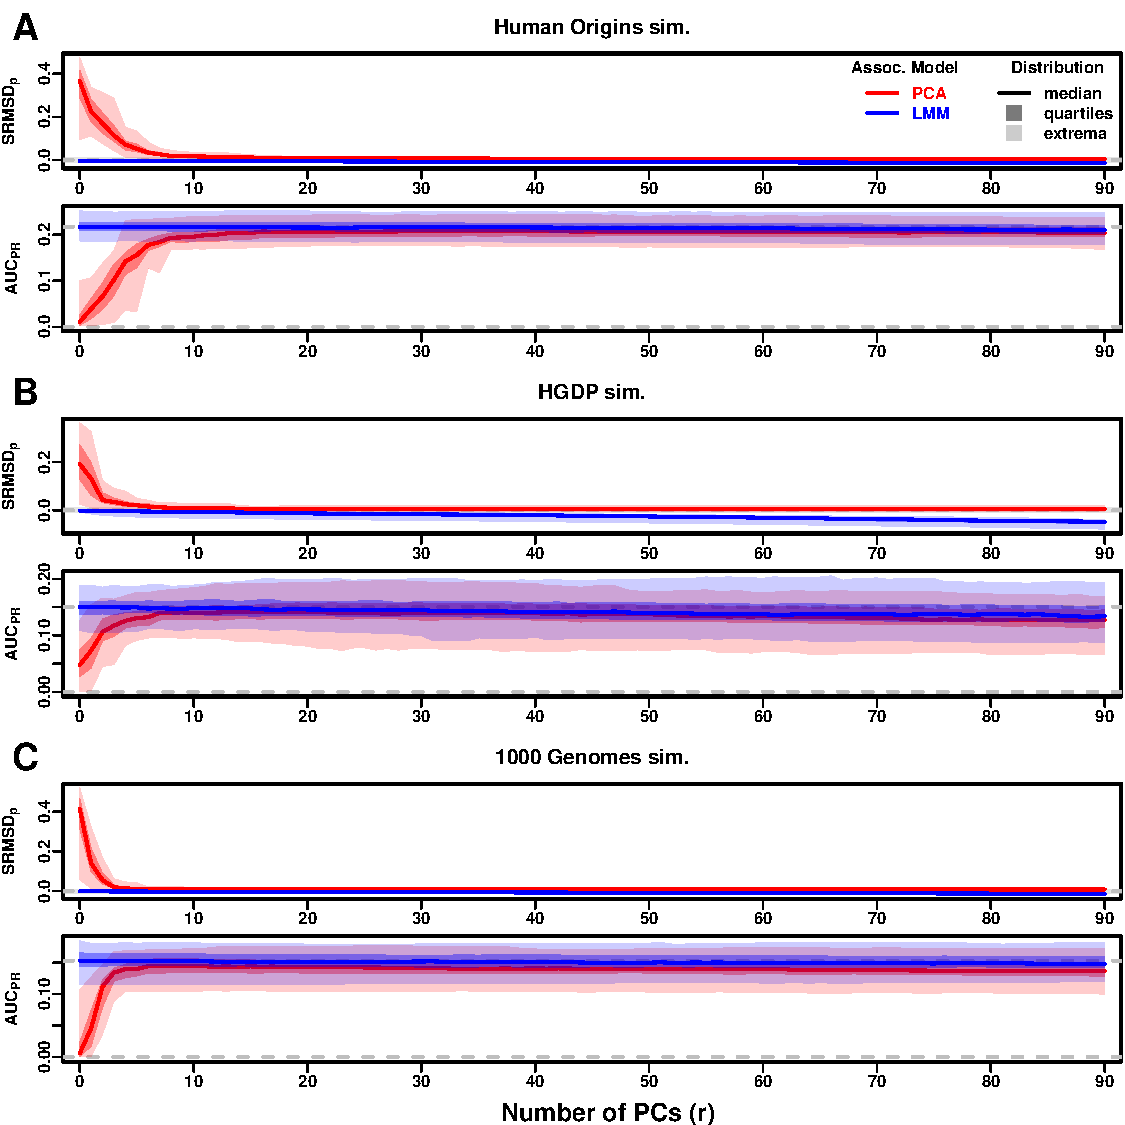
\includegraphics[width=\textwidth,height=\textheight,keepaspectratio]{rmsd-auc-real-sim.pdf}
  \caption{
    {\small 
      {\bf Evaluations in tree simulations fit to human data.}
      Traits simulated from RC model, otherwise the same as \cref{fig:rmsd-auc-real-sim}.
    }
  }
  \label{fig:rmsd-auc-real-sim-rc}
\end{figure}

\begin{figure}[hp!]
  \centering
  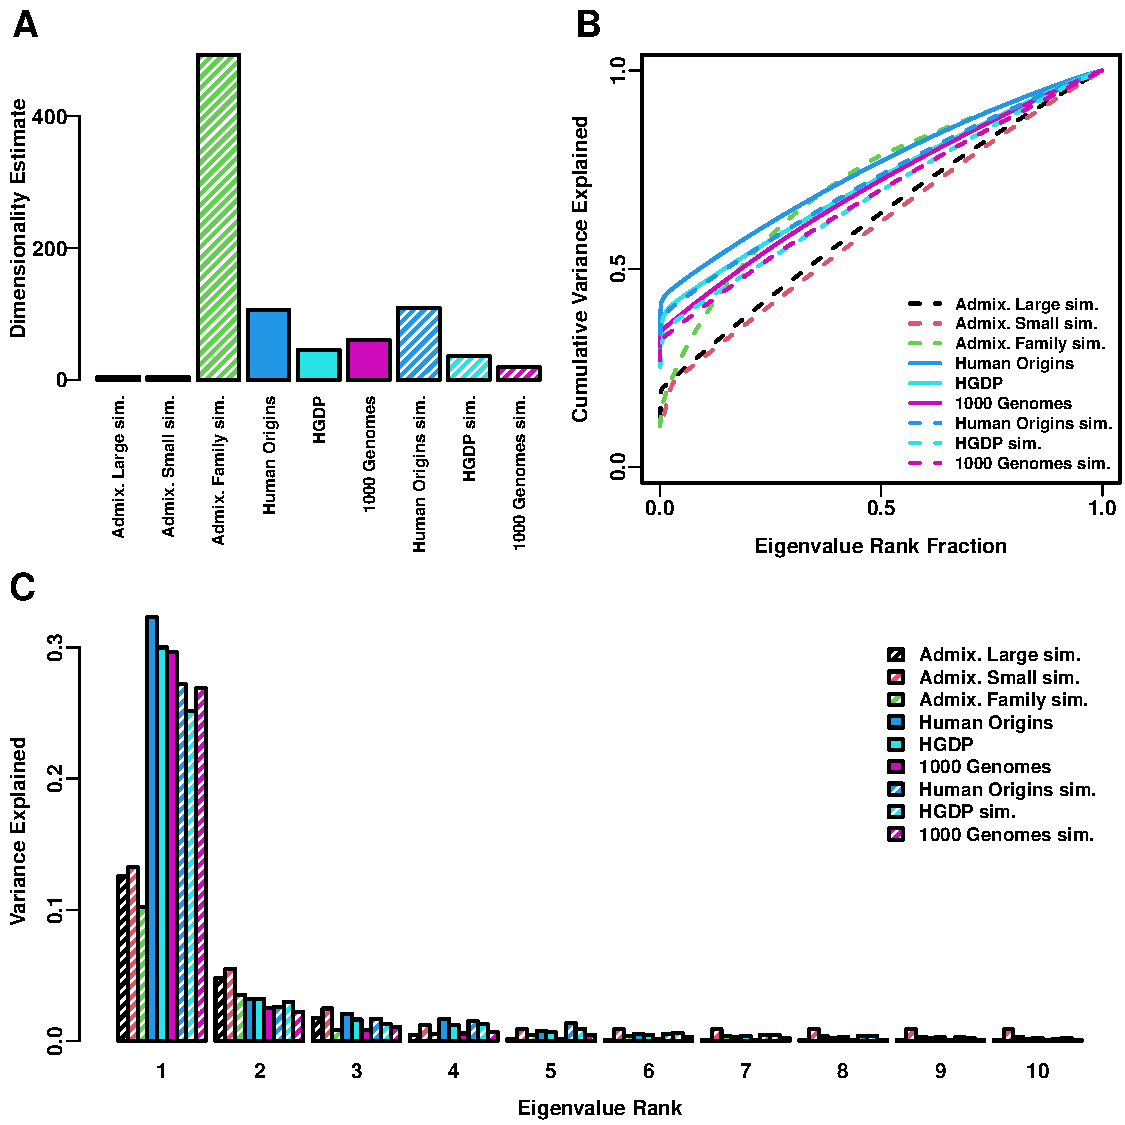
\includegraphics[width=\textwidth]{eigen.pdf}
  \caption{
    {\bf Estimated dimensionality of datasets.}
    \textbf{A.}
    Kinship dimensionalities estimated with the Tracy-Widom test with $p < 0.01$.
    \textbf{B.}
    Cumulative variance explained versus eigenvalue rank fraction.
    \textbf{C.}
    Variance explained by first 10 eigenvalues.
  }
  \label{fig:eigen}
\end{figure}

\clearpage

\section{Supplementary tables}

\begin{table}[hb!]
  \centering
  \footnotesize
  \caption{
    \textbf{Dataset sizes after 4th degree relative filter.}
  }
  \label{tab:king_cutoff}
  % read and automatically format data from a TSV file!
  \sisetup{ table-format = 2, table-number-alignment = right }
  \csvreader[
  tabular = {lSSS},
  separator = tab,
  table head = \toprule Dataset & {Loci ($m$)} & {Ind.~($n$)} & {Ind. removed (\%)} \\\midrule,
  late after last line = \\\bottomrule
  ]{../data/dimensions_king-cutoff-4.txt}{}{\csvlinetotablerow}
\end{table}


\end{document}